
%% bare_jrnl_compsoc.tex
%% V1.4b
%% 2015/08/26
%% by Michael Shell
%% See:
%% http://www.michaelshell.org/
%% for current contact information.
%%
%% This is a skeleton file demonstrating the use of IEEEtran.cls
%% (requires IEEEtran.cls version 1.8b or later) with an IEEE
%% Computer Society journal paper.
%%
%% Support sites:
%% http://www.michaelshell.org/tex/ieeetran/
%% http://www.ctan.org/pkg/ieeetran
%% and
%% http://www.ieee.org/

%%*************************************************************************
%% Legal Notice:
%% This code is offered as-is without any warranty either expressed or
%% implied; without even the implied warranty of MERCHANTABILITY or
%% FITNESS FOR A PARTICULAR PURPOSE! 
%% User assumes all risk.
%% In no event shall the IEEE or any contributor to this code be liable for
%% any damages or losses, including, but not limited to, incidental,
%% consequential, or any other damages, resulting from the use or misuse
%% of any information contained here.
%%
%% All comments are the opinions of their respective authors and are not
%% necessarily endorsed by the IEEE.
%%
%% This work is distributed under the LaTeX Project Public License (LPPL)
%% ( http://www.latex-project.org/ ) version 1.3, and may be freely used,
%% distributed and modified. A copy of the LPPL, version 1.3, is included
%% in the base LaTeX documentation of all distributions of LaTeX released
%% 2003/12/01 or later.
%% Retain all contribution notices and credits.
%% ** Modified files should be clearly indicated as such, including  **
%% ** renaming them and changing author support contact information. **
%%*************************************************************************


% *** Authors should verify (and, if needed, correct) their LaTeX system  ***
% *** with the testflow diagnostic prior to trusting their LaTeX platform ***
% *** with production work. The IEEE's font choices and paper sizes can   ***
% *** trigger bugs that do not appear when using other class files.       ***                          ***
% The testflow support page is at:
% http://www.michaelshell.org/tex/testflow/


\documentclass[10pt,journal,compsoc]{IEEEtran}
%
% If IEEEtran.cls has not been installed into the LaTeX system files,
% manually specify the path to it like:
% \documentclass[10pt,journal,compsoc]{../sty/IEEEtran}





% Some very useful LaTeX packages include:
% (uncomment the ones you want to load)


% *** MISC UTILITY PACKAGES ***
%
%\usepackage{ifpdf}
% Heiko Oberdiek's ifpdf.sty is very useful if you need conditional
% compilation based on whether the output is pdf or dvi.
% usage:
% \ifpdf
%   % pdf code
% \else
%   % dvi code
% \fi
% The latest version of ifpdf.sty can be obtained from:
% http://www.ctan.org/pkg/ifpdf
% Also, note that IEEEtran.cls V1.7 and later provides a builtin
% \ifCLASSINFOpdf conditional that works the same way.
% When switching from latex to pdflatex and vice-versa, the compiler may
% have to be run twice to clear warning/error messages.






% *** CITATION PACKAGES ***
%
\ifCLASSOPTIONcompsoc
  % IEEE Computer Society needs nocompress option
  % requires cite.sty v4.0 or later (November 2003)
  \usepackage[nocompress]{cite}
\else
  % normal IEEE
  \usepackage{cite}
\fi
% cite.sty was written by Donald Arseneau
% V1.6 and later of IEEEtran pre-defines the format of the cite.sty package
% \cite{} output to follow that of the IEEE. Loading the cite package will
% result in citation numbers being automatically sorted and properly
% "compressed/ranged". e.g., [1], [9], [2], [7], [5], [6] without using
% cite.sty will become [1], [2], [5]--[7], [9] using cite.sty. cite.sty's
% \cite will automatically add leading space, if needed. Use cite.sty's
% noadjust option (cite.sty V3.8 and later) if you want to turn this off
% such as if a citation ever needs to be enclosed in parenthesis.
% cite.sty is already installed on most LaTeX systems. Be sure and use
% version 5.0 (2009-03-20) and later if using hyperref.sty.
% The latest version can be obtained at:
% http://www.ctan.org/pkg/cite
% The documentation is contained in the cite.sty file itself.
%
% Note that some packages require special options to format as the Computer
% Society requires. In particular, Computer Society  papers do not use
% compressed citation ranges as is done in typical IEEE papers
% (e.g., [1]-[4]). Instead, they list every citation separately in order
% (e.g., [1], [2], [3], [4]). To get the latter we need to load the cite
% package with the nocompress option which is supported by cite.sty v4.0
% and later. Note also the use of a CLASSOPTION conditional provided by
% IEEEtran.cls V1.7 and later.





% *** GRAPHICS RELATED PACKAGES ***
%
\ifCLASSINFOpdf
  % \usepackage[pdftex]{graphicx}
  % declare the path(s) where your graphic files are
  % \graphicspath{{../pdf/}{../jpeg/}}
  % and their extensions so you won't have to specify these with
  % every instance of \includegraphics
  % \DeclareGraphicsExtensions{.pdf,.jpeg,.png}
\else
  % or other class option (dvipsone, dvipdf, if not using dvips). graphicx
  % will default to the driver specified in the system graphics.cfg if no
  % driver is specified.
  % \usepackage[dvips]{graphicx}
  % declare the path(s) where your graphic files are
  % \graphicspath{{../eps/}}
  % and their extensions so you won't have to specify these with
  % every instance of \includegraphics
  % \DeclareGraphicsExtensions{.eps}
\fi
% graphicx was written by David Carlisle and Sebastian Rahtz. It is
% required if you want graphics, photos, etc. graphicx.sty is already
% installed on most LaTeX systems. The latest version and documentation
% can be obtained at: 
% http://www.ctan.org/pkg/graphicx
% Another good source of documentation is "Using Imported Graphics in
% LaTeX2e" by Keith Reckdahl which can be found at:
% http://www.ctan.org/pkg/epslatex
%
% latex, and pdflatex in dvi mode, support graphics in encapsulated
% postscript (.eps) format. pdflatex in pdf mode supports graphics
% in .pdf, .jpeg, .png and .mps (metapost) formats. Users should ensure
% that all non-photo figures use a vector format (.eps, .pdf, .mps) and
% not a bitmapped formats (.jpeg, .png). The IEEE frowns on bitmapped formats
% which can result in "jaggedy"/blurry rendering of lines and letters as
% well as large increases in file sizes.
%
% You can find documentation about the pdfTeX application at:
% http://www.tug.org/applications/pdftex






% *** MATH PACKAGES ***
%
%\usepackage{amsmath}
% A popular package from the American Mathematical Society that provides
% many useful and powerful commands for dealing with mathematics.
%
% Note that the amsmath package sets \interdisplaylinepenalty to 10000
% thus preventing page breaks from occurring within multiline equations. Use:
%\interdisplaylinepenalty=2500
% after loading amsmath to restore such page breaks as IEEEtran.cls normally
% does. amsmath.sty is already installed on most LaTeX systems. The latest
% version and documentation can be obtained at:
% http://www.ctan.org/pkg/amsmath





% *** SPECIALIZED LIST PACKAGES ***
%
%\usepackage{algorithmic}
% algorithmic.sty was written by Peter Williams and Rogerio Brito.
% This package provides an algorithmic environment fo describing algorithms.
% You can use the algorithmic environment in-text or within a figure
% environment to provide for a floating algorithm. Do NOT use the algorithm
% floating environment provided by algorithm.sty (by the same authors) or
% algorithm2e.sty (by Christophe Fiorio) as the IEEE does not use dedicated
% algorithm float types and packages that provide these will not provide
% correct IEEE style captions. The latest version and documentation of
% algorithmic.sty can be obtained at:
% http://www.ctan.org/pkg/algorithms
% Also of interest may be the (relatively newer and more customizable)
% algorithmicx.sty package by Szasz Janos:
% http://www.ctan.org/pkg/algorithmicx




% *** ALIGNMENT PACKAGES ***
%
%\usepackage{array}
% Frank Mittelbach's and David Carlisle's array.sty patches and improves
% the standard LaTeX2e array and tabular environments to provide better
% appearance and additional user controls. As the default LaTeX2e table
% generation code is lacking to the point of almost being broken with
% respect to the quality of the end results, all users are strongly
% advised to use an enhanced (at the very least that provided by array.sty)
% set of table tools. array.sty is already installed on most systems. The
% latest version and documentation can be obtained at:
% http://www.ctan.org/pkg/array


% IEEEtran contains the IEEEeqnarray family of commands that can be used to
% generate multiline equations as well as matrices, tables, etc., of high
% quality.




% *** SUBFIGURE PACKAGES ***
%\ifCLASSOPTIONcompsoc
%  \usepackage[caption=false,font=footnotesize,labelfont=sf,textfont=sf]{subfig}
%\else
%  \usepackage[caption=false,font=footnotesize]{subfig}
%\fi
% subfig.sty, written by Steven Douglas Cochran, is the modern replacement
% for subfigure.sty, the latter of which is no longer maintained and is
% incompatible with some LaTeX packages including fixltx2e. However,
% subfig.sty requires and automatically loads Axel Sommerfeldt's caption.sty
% which will override IEEEtran.cls' handling of captions and this will result
% in non-IEEE style figure/table captions. To prevent this problem, be sure
% and invoke subfig.sty's "caption=false" package option (available since
% subfig.sty version 1.3, 2005/06/28) as this is will preserve IEEEtran.cls
% handling of captions.
% Note that the Computer Society format requires a sans serif font rather
% than the serif font used in traditional IEEE formatting and thus the need
% to invoke different subfig.sty package options depending on whether
% compsoc mode has been enabled.
%
% The latest version and documentation of subfig.sty can be obtained at:
% http://www.ctan.org/pkg/subfig




% *** FLOAT PACKAGES ***
%
%\usepackage{fixltx2e}
% fixltx2e, the successor to the earlier fix2col.sty, was written by
% Frank Mittelbach and David Carlisle. This package corrects a few problems
% in the LaTeX2e kernel, the most notable of which is that in current
% LaTeX2e releases, the ordering of single and double column floats is not
% guaranteed to be preserved. Thus, an unpatched LaTeX2e can allow a
% single column figure to be placed prior to an earlier double column
% figure.
% Be aware that LaTeX2e kernels dated 2015 and later have fixltx2e.sty's
% corrections already built into the system in which case a warning will
% be issued if an attempt is made to load fixltx2e.sty as it is no longer
% needed.
% The latest version and documentation can be found at:
% http://www.ctan.org/pkg/fixltx2e


%\usepackage{stfloats}
% stfloats.sty was written by Sigitas Tolusis. This package gives LaTeX2e
% the ability to do double column floats at the bottom of the page as well
% as the top. (e.g., "\begin{figure*}[!b]" is not normally possible in
% LaTeX2e). It also provides a command:
%\fnbelowfloat
% to enable the placement of footnotes below bottom floats (the standard
% LaTeX2e kernel puts them above bottom floats). This is an invasive package
% which rewrites many portions of the LaTeX2e float routines. It may not work
% with other packages that modify the LaTeX2e float routines. The latest
% version and documentation can be obtained at:
% http://www.ctan.org/pkg/stfloats
% Do not use the stfloats baselinefloat ability as the IEEE does not allow
% \baselineskip to stretch. Authors submitting work to the IEEE should note
% that the IEEE rarely uses double column equations and that authors should try
% to avoid such use. Do not be tempted to use the cuted.sty or midfloat.sty
% packages (also by Sigitas Tolusis) as the IEEE does not format its papers in
% such ways.
% Do not attempt to use stfloats with fixltx2e as they are incompatible.
% Instead, use Morten Hogholm'a dblfloatfix which combines the features
% of both fixltx2e and stfloats:
%
% \usepackage{dblfloatfix}
% The latest version can be found at:
% http://www.ctan.org/pkg/dblfloatfix




%\ifCLASSOPTIONcaptionsoff
%  \usepackage[nomarkers]{endfloat}
% \let\MYoriglatexcaption\caption
% \renewcommand{\caption}[2][\relax]{\MYoriglatexcaption[#2]{#2}}
%\fi
% endfloat.sty was written by James Darrell McCauley, Jeff Goldberg and 
% Axel Sommerfeldt. This package may be useful when used in conjunction with 
% IEEEtran.cls'  captionsoff option. Some IEEE journals/societies require that
% submissions have lists of figures/tables at the end of the paper and that
% figures/tables without any captions are placed on a page by themselves at
% the end of the document. If needed, the draftcls IEEEtran class option or
% \CLASSINPUTbaselinestretch interface can be used to increase the line
% spacing as well. Be sure and use the nomarkers option of endfloat to
% prevent endfloat from "marking" where the figures would have been placed
% in the text. The two hack lines of code above are a slight modification of
% that suggested by in the endfloat docs (section 8.4.1) to ensure that
% the full captions always appear in the list of figures/tables - even if
% the user used the short optional argument of \caption[]{}.
% IEEE papers do not typically make use of \caption[]'s optional argument,
% so this should not be an issue. A similar trick can be used to disable
% captions of packages such as subfig.sty that lack options to turn off
% the subcaptions:
% For subfig.sty:
% \let\MYorigsubfloat\subfloat
% \renewcommand{\subfloat}[2][\relax]{\MYorigsubfloat[]{#2}}
% However, the above trick will not work if both optional arguments of
% the \subfloat command are used. Furthermore, there needs to be a
% description of each subfigure *somewhere* and endfloat does not add
% subfigure captions to its list of figures. Thus, the best approach is to
% avoid the use of subfigure captions (many IEEE journals avoid them anyway)
% and instead reference/explain all the subfigures within the main caption.
% The latest version of endfloat.sty and its documentation can obtained at:
% http://www.ctan.org/pkg/endfloat
%
% The IEEEtran \ifCLASSOPTIONcaptionsoff conditional can also be used
% later in the document, say, to conditionally put the References on a 
% page by themselves.




% *** PDF, URL AND HYPERLINK PACKAGES ***
%
%\usepackage{url}
% url.sty was written by Donald Arseneau. It provides better support for
% handling and breaking URLs. url.sty is already installed on most LaTeX
% systems. The latest version and documentation can be obtained at:
% http://www.ctan.org/pkg/url
% Basically, \url{my_url_here}.





% *** Do not adjust lengths that control margins, column widths, etc. ***
% *** Do not use packages that alter fonts (such as pslatex).         ***
% There should be no need to do such things with IEEEtran.cls V1.6 and later.
% (Unless specifically asked to do so by the journal or conference you plan
% to submit to, of course. )


% correct bad hyphenation here
%\hyphenation{op-tical net-works semi-conduc-tor}
\usepackage{graphicx}
\usepackage{epstopdf}
\usepackage{balance}  % for  \balance command ON LAST PAGE  (only there!)
%\usepackage[utf8]{inputenc}
\usepackage{color}
%\usepackage{fullpage}
\usepackage{enumerate}
\usepackage{xcolor,listings}
\usepackage{url}
\usepackage[normalem]{ulem}
\usepackage{amsmath,amsthm,amsfonts}
\usepackage[vlined]{algorithm2e}

\usepackage{subfigure}
%\usepackage{MinionPro}
\usepackage{multirow}
\usepackage{varwidth}
\usepackage{verbatim}
\usepackage{xspace}
\usepackage{paralist}
\usepackage[noend]{algpseudocode}
\usepackage{flushend}


\newcommand{\summaryS}[1]{
 \begin{flushleft}
               \vspace{-5pt}
               \fbox{%
               %\setstretch{0.95}
               \parbox{0.95\linewidth}{%
               \vspace{-2pt}
                 {\small {\em Summary:} #1}
                 \vspace{-2pt}
                 }
               }
 \vspace{-7pt}
 \end{flushleft}
}

\newcommand{\Eg}{{\itshape E.g.}, }
\newcommand{\eg}{{\itshape e.g.}, }
\newcommand{\ie}{{\itshape i.e.}, }
\newcommand{\xie}{{\itshape I.e.}, }
\newcommand{\etc}{{\itshape etc.\/}}

\newcommand{\squishlist}{
  \begin{list}{$\bullet$}
           { \setlength{\itemsep}{0pt}
             \setlength{\parsep}{2pt}
             \setlength{\topsep}{2pt}
             \setlength{\partopsep}{0pt}
           }
}
\newcommand{\squishend}{\end{list}}


\newcommand{\squishenum}{
       \begin{enumerate}
               { \setlength{\itemsep}{-50pt}
                       \setlength{\parsep}{0pt}
                       \setlength{\topsep}{0pt}
                       \setlength{\partopsep}{0pt}
               }
       }
       \newcommand{\squishenumend}{\end{enumerate}}


\newcommand{\infovis}[1]{\textcolor{red}{\textbf{INFOVIS}: #1}}
\newcommand{\saj}[1]{\textcolor{teal}{#1}}
\newcommand{\new}[1]{\textcolor{blue}{#1}}

\newcommand{\agp}[1]{\textcolor{magenta}{AGP: #1}}
\newcommand{\kgk}[1]{\textcolor{magenta}{#1}}
\newcommand{\introNew}[1]{{#1}}
\newcommand{\introOld}[1]{}
\newcommand{\toappendix}[1]{}

\newenvironment{paraenum}{\begin{inparaenum}[\itshape (a)\upshape]}{\end{inparaenum}}
\newcommand{\para}[1]{\vspace{2pt} \noindent {\bfseries #1.}}
\newcommand{\response}[1]{``\emph{#1}''}
\newcommand{\system}{{\scshape NOAH}\xspace}
\newcommand{\noah}{{\scshape NOAH}\xspace}
\newcommand{\cmpA}{{compare~($2$)}\xspace}
\newcommand{\cmpB}{{compare~($N$)}\xspace}
\newcommand{\cut}[1]{}
\newcommand{\additional}[1]{}
\newcommand{\stitle}[1]{\vspace{0.2em}\noindent\textbf{#1}}
\newcommand{\ttitle}[1]{\vspace{0.2em}\noindent\textbf{#1}}
\newcommand{\emtitle}[1]{\vspace{0.2em}\noindent\underline{\emph{#1}}}
\newcommand{\code}[1]{\texttt{\small #1}}

\newcommand{\ta}[1]{\vspace{-3pt}\begin{framed}\vspace{-5pt}\noindent\textit{\underline{Takeaway \thetctr\stepcounter{tctr}:} #1}\vspace{-5pt}\end{framed}\vspace{-3pt}}

\newcommand{\boxy}[1]{\vspace{-3pt}\begin{framed}\vspace{-5pt}\noindent#1\vspace{-7pt}\end{framed}\vspace{-5pt}}

\begin{document}
%
% paper title
% Titles are generally capitalized except for words such as a, an, and, as,
% at, but, by, for, in, nor, of, on, or, the, to and up, which are usually
% not capitalized unless they are the first or last word of the title.
% Linebreaks \\ can be used within to get better formatting as desired.
% Do not put math or special symbols in the title.

\title{Extending Spreadsheets to Support Seamless Navigation at Scale}
%
%
% author names and IEEE memberships
% note positions of commas and nonbreaking spaces ( ~ ) LaTeX will not break
% a structure at a ~ so this keeps an author's name from being broken across
% two lines.
% use \thanks{} to gain access to the first footnote area
% a separate \thanks must be used for each paragraph as LaTeX2e's \thanks
% was not built to handle multiple paragraphs
%
%
%\IEEEcompsocitemizethanks is a special \thanks that produces the bulleted
% lists the Computer Society journals use for "first footnote" author
% affiliations. Use \IEEEcompsocthanksitem which works much like \item
% for each affiliation group. When not in compsoc mode,
% \IEEEcompsocitemizethanks becomes like \thanks and
% \IEEEcompsocthanksitem becomes a line break with idention. This
% facilitates dual compilation, although admittedly the differences in the
% desired content of \author between the different types of papers makes a
% one-size-fits-all approach a daunting prospect. For instance, compsoc 
% journal papers have the author affiliations above the "Manuscript
% received ..."  text while in non-compsoc journals this is reversed. Sigh.
%Pingjing Yang..py2, Zhaoyuan Su..zsu7, Kevin Chen-Chuan Chang..kcchang, 
\author{Sajjadur Rahman, Mangesh Bendre, Yuyang Liu, Shichu Zhu, Karrie Karahalios, and Aditya Parameswaran
\IEEEcompsocitemizethanks{\IEEEcompsocthanksitem Sajjadur Rahman, Yuyang Liu, Shichu Zhu and Karrie Karahalios are with the Department of Computer Science at University of Illinois, Urbana-Champaign. Email: \{srahman7, yuyangl2, szhu28, kkarahal\}@illinois.edu.
\IEEEcompsocthanksitem Mangesh Bendre is with VISA Research. Email: mbendre@visa.com.
\IEEEcompsocthanksitem Aditya Parameswaran is with the I School and EECS at the University of California, Berkeley. Email: adityagp@berkeley.edu.
}% <-this % stops an unwanted space
%\thanks{Manuscript received April 19, 2005; revised August 26, 2015.}
}

% note the % following the last \IEEEmembership and also \thanks - 
% these prevent an unwanted space from occurring between the last author name
% and the end of the author line. i.e., if you had this:
% 
% \author{....lastname \thanks{...} \thanks{...} }
%                     ^------------^------------^----Do not want these spaces!
%
% a space would be appended to the last name and could cause every name on that
% line to be shifted left slightly. This is one of those "LaTeX things". For
% instance, "\textbf{A} \textbf{B}" will typeset as "A B" not "AB". To get
% "AB" then you have to do: "\textbf{A}\textbf{B}"
% \thanks is no different in this regard, so shield the last } of each \thanks
% that ends a line with a % and do not let a space in before the next \thanks.
% Spaces after \IEEEmembership other than the last one are OK (and needed) as
% you are supposed to have spaces between the names. For what it is worth,
% this is a minor point as most people would not even notice if the said evil
% space somehow managed to creep in.



% The paper headers
%\markboth{Journal of \LaTeX\ Class Files,~Vol.~14, No.~8, August~2015}%
%{Shell \MakeLowercase{\textit{et al.}}: Bare Demo of IEEEtran.cls for Computer Society Journals}
% The only time the second header will appear is for the odd numbered pages
% after the title page when using the twoside option.
% 
% *** Note that you probably will NOT want to include the author's ***
% *** name in the headers of peer review papers.                   ***
% You can use \ifCLASSOPTIONpeerreview for conditional compilation here if
% you desire.



% The publisher's ID mark at the bottom of the page is less important with
% Computer Society journal papers as those publications place the marks
% outside of the main text columns and, therefore, unlike regular IEEE
% journals, the available text space is not reduced by their presence.
% If you want to put a publisher's ID mark on the page you can do it like
% this:
%\IEEEpubid{0000--0000/00\$00.00~\copyright~2015 IEEE}
% or like this to get the Computer Society new two part style.
%\IEEEpubid{\makebox[\columnwidth]{\hfill 0000--0000/00/\$00.00~\copyright~2015 IEEE}%
%\hspace{\columnsep}\makebox[\columnwidth]{Published by the IEEE Computer Society\hfill}}
% Remember, if you use this you must call \IEEEpubidadjcol in the second
% column for its text to clear the IEEEpubid mark (Computer Society jorunal
% papers don't need this extra clearance.)



% use for special paper notices
%\IEEEspecialpapernotice{(Invited Paper)}



% for Computer Society papers, we must declare the abstract and index terms
% PRIOR to the title within the \IEEEtitleabstractindextext IEEEtran
% command as these need to go into the title area created by \maketitle.
% As a general rule, do not put math, special symbols or citations
% in the abstract or keywords.
%!TEX root = main.tex


\section*{Resubmission of InfoVis 2019 submission ``Extending Spreadsheets to Support Seamless
Navigation at Scale'' to TVCG}

A previous version of this paper was submitted to InfoVis 2019. This version was rejected as the paper co-chairs deemed that revising the paper would require more time than allocated to meet reviewer expectations. The paper co-chairs mentioned the following: ``\textit{We particularly encourage such revisions where submissions were positively received by reviewers, but the revisions required were deemed to be beyond the scope of the conference review cycle. If you address the issues raised and subsequently submit to TVCG, please make reference to this  InfoVis submission and include a description of how you addressed the InfoVis reviewers' comments.}'' The entire set of reviews are attached. In particular, the reviewers asked for the following changes for a revision: 
\begin{itemize}
    \item[\textbf{C1:}] More clearly articulate the merits over alternative tools, such as Keshif. 
     \item[\textbf{C2:}] Convincingly explain the design choice around the binning mechanism or revise
    that approach.
    \item[\textbf{C3:}] Justify the choice of comparing with Excel and note the limitations of that
    approach.
     \item[\textbf{C4:}] Better justify the choice of tasks in the study. 
     \item[\textbf{C5:}] Explain the choice of the four research questions.
     \item[\textbf{C6:}] Provide more details about the study, including reporting intra-participant
    differences.
\end{itemize} 
\new{We thank the reviewers and meta-reviewer for their detailed,
constructive feedback. 
Taking this feedback into account, 
we have spent the last four months 
preparing a revised version of this paper.
We believe the paper is substantially
stronger as a result. 
Every section in the paper has been revised;
the changes are highlighted in blue.
We briefly describe the changes to each section
before returning to the changes required in the revision 
({\bf C1}--{\bf C6}).
\subsection*{Changes Organized by Section}
\begin{itemize}
	\leftmargin=25pt \rightmargin=0pt \labelsep=5pt \labelwidth=20pt \itemindent=0pt \listparindent=0pt \topsep=0pt plus 2pt minus 4pt \partopsep=0pt plus 1pt minus 1pt \parsep=0pt plus 1pt \itemsep=\parsep
\item 
In Section~\ref{sec:intro}, we now cite
work that highlights the widespread adoption
of spreadsheets even among users of 
advanced enterprise solutions, further justifying 
why we focused on addressing navigation challenges within
spreadsheets. In fact, recent 
debate within the visualization community following
VIS 2019 also echoes this view\footnote{https://twitter.com/FILWD/status/1187411664611749888}---instead of designing a new sophisticated tool from scratch that 
may cater to a small population, 
we aim to enhance the user experience for
existing spreadsheet tools
with nearly a billion users.
Furthermore, in Section~\ref{sec:intro},  
the definitions of spreadsheet 
interactions like scrolling and steering have been augmented, and 
we now clearly articulate the challenges of 
designing a general-purpose plug-in for spreadsheets.
\item 
In Section~\ref{sec:usage}, 
our usage scenario has been substantially revised 
using Brehmer and Munzner's typology~\cite{brehmer2013multi} to
clarify the scope of tasks supported by 
a \noah-enhanced spreadsheet; our new Table~\ref{tab:scope}
provides use-cases supported within \noah
for each category.
\item
In Section~\ref{sec:related},
we now clearly
articulate the differences in goals
of spreadsheets and tabular data analysis tools (TDA),
further justifying our choice of Excel,
the most widely used spreadsheet tool,
as our baseline in the evaluation study.
\item 
In Section~\ref{sec:design},
we now explain the  
third design consideration 
for \noah more clearly
(\textbf{DC3})---focusing on motivating the binning
mechanism. 
\item In Section~\ref{sec:ui}, 
we now justify why we are developing a 
multi-granularity overview,
and explain why 
we opted for histograms as an overview representation. 
\item 
In Section~\ref{sec:study}, 
we further clarified the goals of our study
and reframed our research questions to 
better reflect those goals. 
Our research questions haven't been substantially altered;
rather, they have been grouped together and made less
ambiguous. In this version,
we now explain our choice
for the quiz tasks and discuss 
three limitations of our study in detail. 
\item Section~\ref{sec:results} has been completely
revamped to better reflect our research questions,
while adding more qualitative observations 
regarding the user experience with \noah. 
We now
include additional analysis results on intra-participant differences. 
\item In Section~\ref{sec:discuss}, we have added a summary of our takeaways from the evaluation study, while discussing additional limitations of \noah and future enhancement opportunities. 
\end{itemize}
\subsection*{Changes Organized by Reviewer Concerns (C1--C6)}
}

\begin{enumerate}
\leftmargin=25pt \rightmargin=0pt \labelsep=5pt \labelwidth=20pt \itemindent=0pt \listparindent=0pt \topsep=0pt plus 2pt minus 4pt \partopsep=0pt plus 1pt minus 1pt \parsep=0pt plus 1pt \itemsep=\parsep

\item \textit{Merits over other tools} (\textbf{C1}): 
\new{Throughout the paper (and especially in 
Sections~\ref{sec:intro}, \ref{sec:related},
and \ref{sec:study}), we have emphasized
that the main contribution of \noah
is its \emph{design as a general-purpose navigation plug-in} 
to any existing spreadsheet system. 
As spreadsheets have a massive user-base, 
enhancing exploration and formula computation 
on large datasets while maintaining 
the spreadsheet look-and-feel as much as possible, 
has the potential to impact hundreds of millions 
of spreadsheet users. 
Most of these users employ spreadsheets 
as their primary data management and analysis 
tool while shunning enterprise solutions 
with more advanced features. 
Therefore, our goal is to develop a 
solution to improve navigation within spreadsheets.
Indeed, we could have tried to enhance navigation
in other tools, such as Keshif, or Tableau, like
the reviewers suggest---but we would be forcing
spreadsheet users to adopt an entirely new tool, something
that they are clearly loath to do.} 

\item \textit{Explanation of the binning mechanism} (\textbf{C2}): 
\new{We now explain our choice
of the binning mechanism in 
the context of the third design consideration (\emph{DC3}), 
as detailed in Section~\ref{sec:design}.
We further expand on this in the blurb titled 
``Why a Multi-granularity Binned Overview'' 
in Section~\ref{sec:ui}.
In brief, we opted for binning to 
provide a clear and concise 
representation of the overall data 
distribution while minimizing user's back 
and forth movement across multiple screens 
during navigation. 
At some level, we do need to limit the number
of values displayed so that the overview
fits on the screen: binning is a natural solution
for that issue. 
\agp{Possibly argue using the immens paper?}
However, we acknowledge limitations 
for this choice for binning categorical data 
and discuss possible solutions 
in Section~\ref{sec:discuss} 
in the context of our user study findings. 
}

\item \textit{Justification of Excel as a Baseline} (\textbf{C2}):
\new{Since our goal is to improve spreadsheet
user experience---and there are very good reasons for doing so,
as outlined in item 1) above---the natural comparison point
is Excel. 
That said, beyond popularity, 
we have provided a thorough justification
for what spreadsheet systems like Excel offer
relative to tabular data analysis tools (TDA),
making it a more appropriate point of comparison.
Our justification for using Excel over 
tabular data analysis (TDA) tools involves 
a) highlighting the appeal of spreadsheets 
among users who shun more advanced enterprise 
tools (Section~\ref{sec:intro}), 
b) identifying the scope of tasks 
supported by spreadsheets and 
TDA tools (Section~\ref{sec:usage} and~\ref{sec:related}), 
c) explaining that the goal of spreadsheets 
is to present the raw data as is, 
amenable to editing, formula computation, and comparison of derived data, all done in-situ,
unlike TDA tools that hide the data 
while providing summarized statistics 
(Section~\ref{sec:related}), and 
d) highlighting the importance of 
addressing the shortcomings of a tool, 
the user base of which far exceeds 
that of TDA tools (Section~\ref{sec:study}). 
}

\item \textit{Enhancing the user study design} 
(\textbf{C4, C5}):
\agp{Revise to clarify where these changes are made
and HOW these changes solve the issue. Just saying
we merged doesn't necessarily address the issue.}
We have added additional 
explanations regarding the goal 
of the study while better articulating 
the research questions, provided a better justification for the choice of the tasks for the study (see Section~\ref{sec:study_design}) and added a detailed discussion on the limitations of the study. \saj{Specifically, we merged a number of research questions that explored how specific features of \noah affected participants' navigation experience into one broad question which explores their overall experience with \noah and its components. Moreover, we have justified the choice of the quiz tasks by a) relating their goals with the scope of tasks supported by spreadsheets (see Section~\ref{sec:usage}), and b) explaining how these tasks can reveal how people may use \noah for spreadsheet navigation. Finally, we have identified two limitations of the study, resulting from the sample size and the study design, which we justify based on the scope of the study.}

\item \textit{Reporting Intra-participant Differences} (\textbf{C6}):
\new{We performed additional analysis of the study data to report intra-participant submission time differences while providing insights on the trends that emerged from analyzing the data: this new analysis can be found in XXX\agp{pls add; insights on trends sounds vague let's be more clear}.} \saj{For the latter, we find that, despite a few exceptions, across all tasks, participants' task submission times were faster using \noah. However, we already obtained similar observations from Figure~\ref{fig:timeBox} in Section~\ref{sec:rq1}. Therefore, we have included the results of the intra-participant analysis in appendix while briefly summarizing its outcomes in Section~\ref{sec:rq1}.}
\end{enumerate}

\IEEEtitleabstractindextext{%
\begin{abstract}
Spreadsheets are one of the most popular tools for
ad-hoc exploration and analysis of data. 
Despite that, exploring and analyzing spreadsheet
datasets that span more than a few screens via operations such as scrolling or issuing formulae,
is often overwhelming for end-users. 
Users easily lose context 
as they explore the data via scrolling and
suffer from cognitive and mechanical burdens
while issuing formulae on 
data spanning multiple screens.
We propose integrating a navigation 
plug-in with spreadsheets 
to support the seamless exploration 
of large datasets that are increasingly
the norm.
Our interface, \noah, developed
using lessons from classical overview+detail interfaces,
embeds a multi-granularity zoomable overview alongside
the spreadsheet. 
Users can employ the overview to 
explore the data 
at various granularities. Furthermore, they can issue formulae over subsets of data without performing
cumbersome scrolling or range selection operations,
enabling users to gain 
a high or low-level perspective of the spreadsheet data.
\noah preserves spreadsheet semantics and look and feel,
while introducing such enhancements.
Our user study demonstrates that 
\noah makes it more intuitive, easier, and faster
to navigate spreadsheet data compared to traditional spreadsheets
like Microsoft Excel, for a variety of navigational tasks; 
participants made $2.5\times$ fewer mistakes in \noah than in Excel
while being twice as fast in completing the tasks.
\end{abstract}

% Note that keywords are not normally used for peerreview papers.
\begin{IEEEkeywords}
Spreadsheet navigation, data exploration, overview+detail, zooming.
\end{IEEEkeywords}}


% make the title area
\maketitle

% To allow for easy dual compilation without having to reenter the
% abstract/keywords data, the \IEEEtitleabstractindextext text will
% not be used in maketitle, but will appear (i.e., to be "transported")
% here as \IEEEdisplaynontitleabstractindextext when the compsoc 
% or transmag modes are not selected <OR> if conference mode is selected 
% - because all conference papers position the abstract like regular
% papers do.
\IEEEdisplaynontitleabstractindextext
% \IEEEdisplaynontitleabstractindextext has no effect when using
% compsoc or transmag under a non-conference mode.



% For peer review papers, you can put extra information on the cover
% page as needed:
% \ifCLASSOPTIONpeerreview
% \begin{center} \bfseries EDICS Category: 3-BBND \end{center}
% \fi
%
% For peerreview papers, this IEEEtran command inserts a page break and
% creates the second title. It will be ignored for other modes.
\IEEEpeerreviewmaketitle

%!TEX root = main.tex

%\IEEEraisesectionheading{\section{Introduction}}
\section{Introduction}
\label{sec:intro}
\new{With a user base of more than  one-tenth of the world's population,
{\bf \em spreadsheets are by far the most popular medium for ad-hoc exploration
and analysis of data}~\cite{excel-users}.} 
\saj{Studies show that information workers prefer to operate on their data within spreadsheets while shunning enterprise solutions 
with more advanced analytical features~\cite{chan1996use,raden2005shedding}. 
One popular joke among those developing business intelligence applications is that  the ``export to excel'' button is the third-most commonly used button from the menu bar, after OK and Cancel~\cite{bakke2016expressive}.}
Spreadsheets enable users to view, structure, and present data
in an intuitive tabular layout, wherein users can map their data and tasks;
this tabular layout is essential to
the popularity of spreadsheets~\cite{nardi1990spreadsheet}.

Using this tabular layout effectively involves
navigation, \ie
{\em ``the process of viewing and manipulating the computer display to
show another portion of the information space''}~\cite{nav-study}.
Navigation is supported
via two unit operations, scrolling and steering.
\saj{Scrolling is the action of moving displayed text or graphics up, down, or across a computer screen, in order to view different parts of the spreadsheet.}
For example, when analyzing data, users may scroll
to compare data across different screens, or to get
a high-level view of the overall spreadsheet.
\saj{Steering, on the other hand, involves clicking the left mouse button and then dragging the mouse pointer through the spreadsheet to select a specific region.} For example, to issue a formula,
users may steer to select
the subset of the data
to be operated on as an argument within the formula.
Most frequently used spreadsheet formulae
require users to perform steering actions~\cite{bradbard2014spreadsheet, lawson2009comparison}.
Overall, both scrolling and steering are crucial as
users navigate spreadsheets to
identify, compare, and summarize data.

\begin{figure*}
     \centering %trim=left bottom right top
  %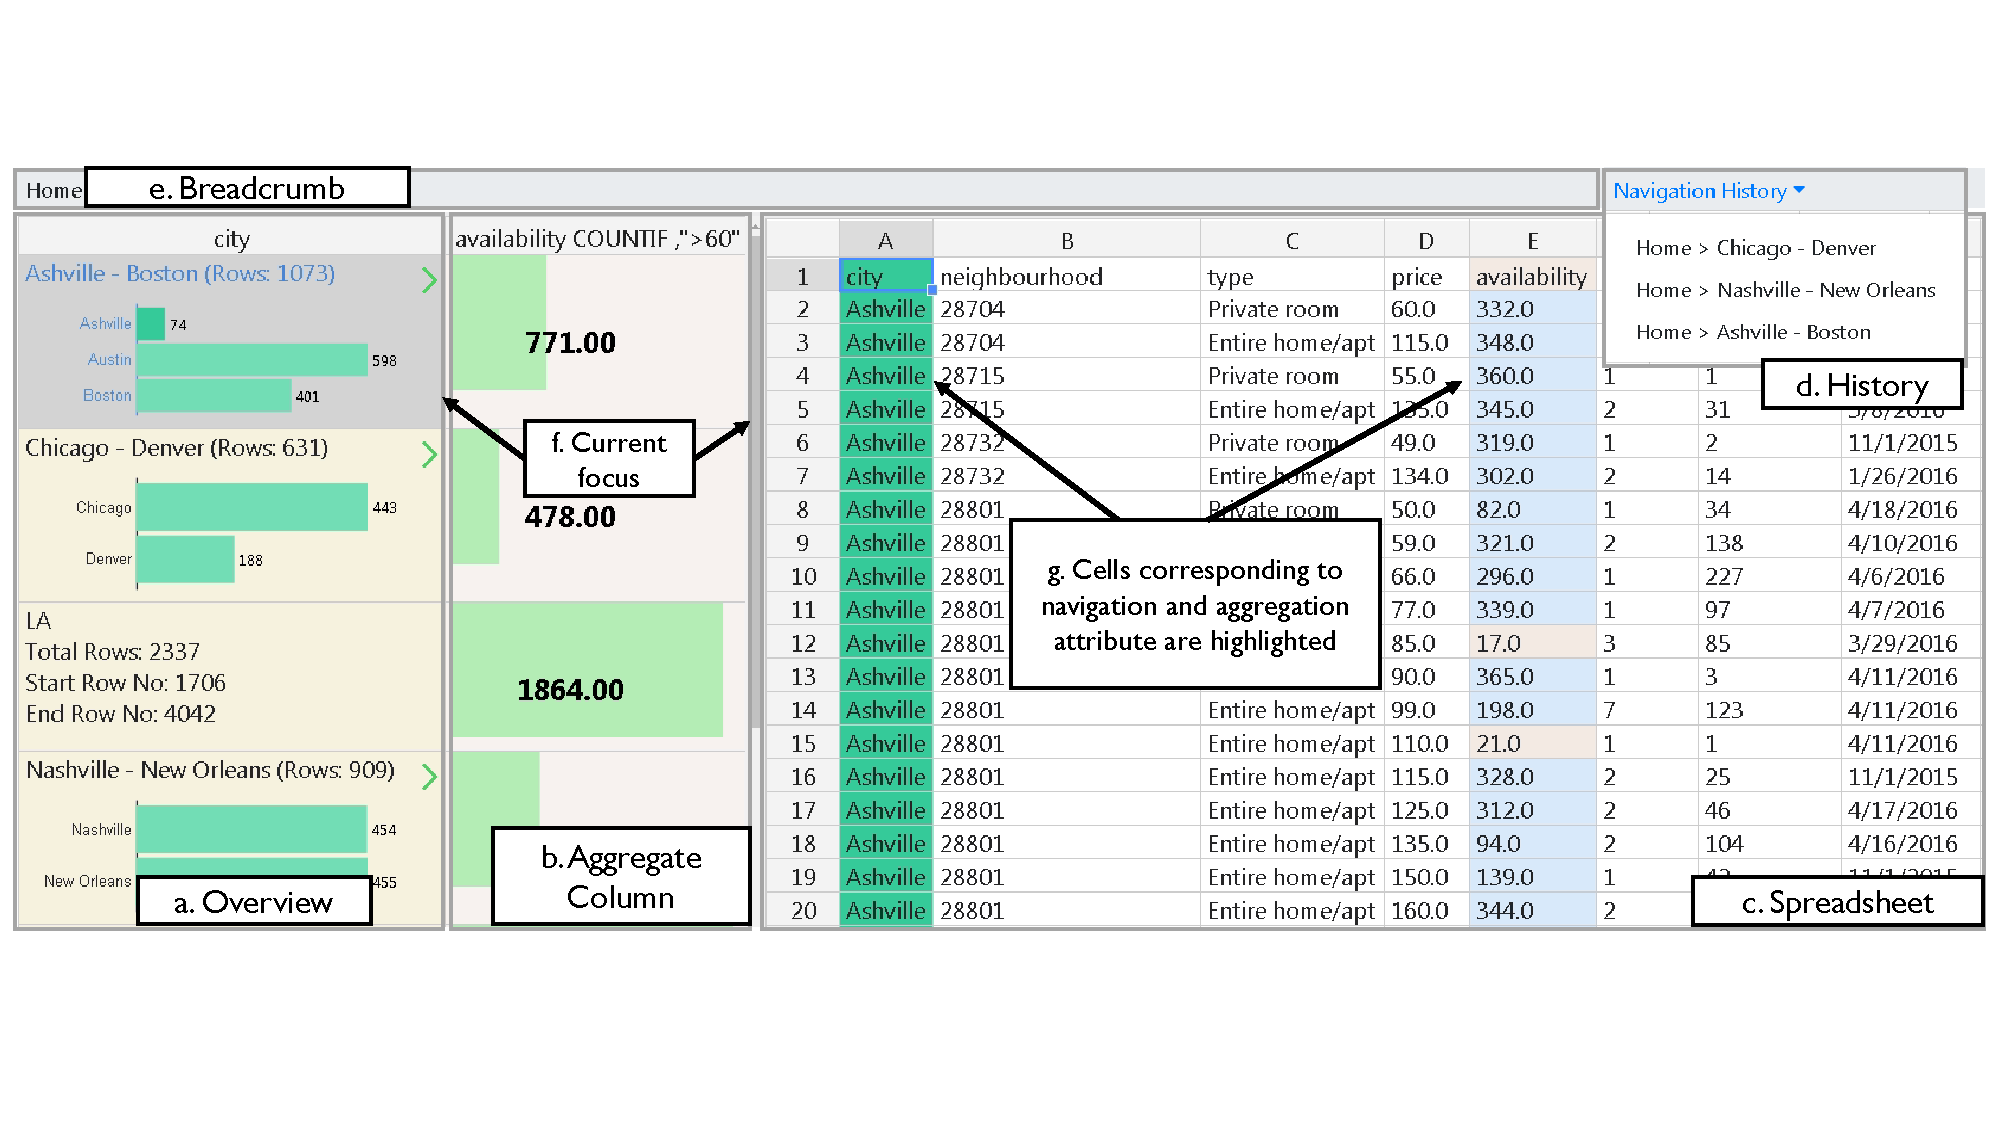
\includegraphics[width=\linewidth,trim={0 95 0 80},clip]{images/navigation.pdf}
  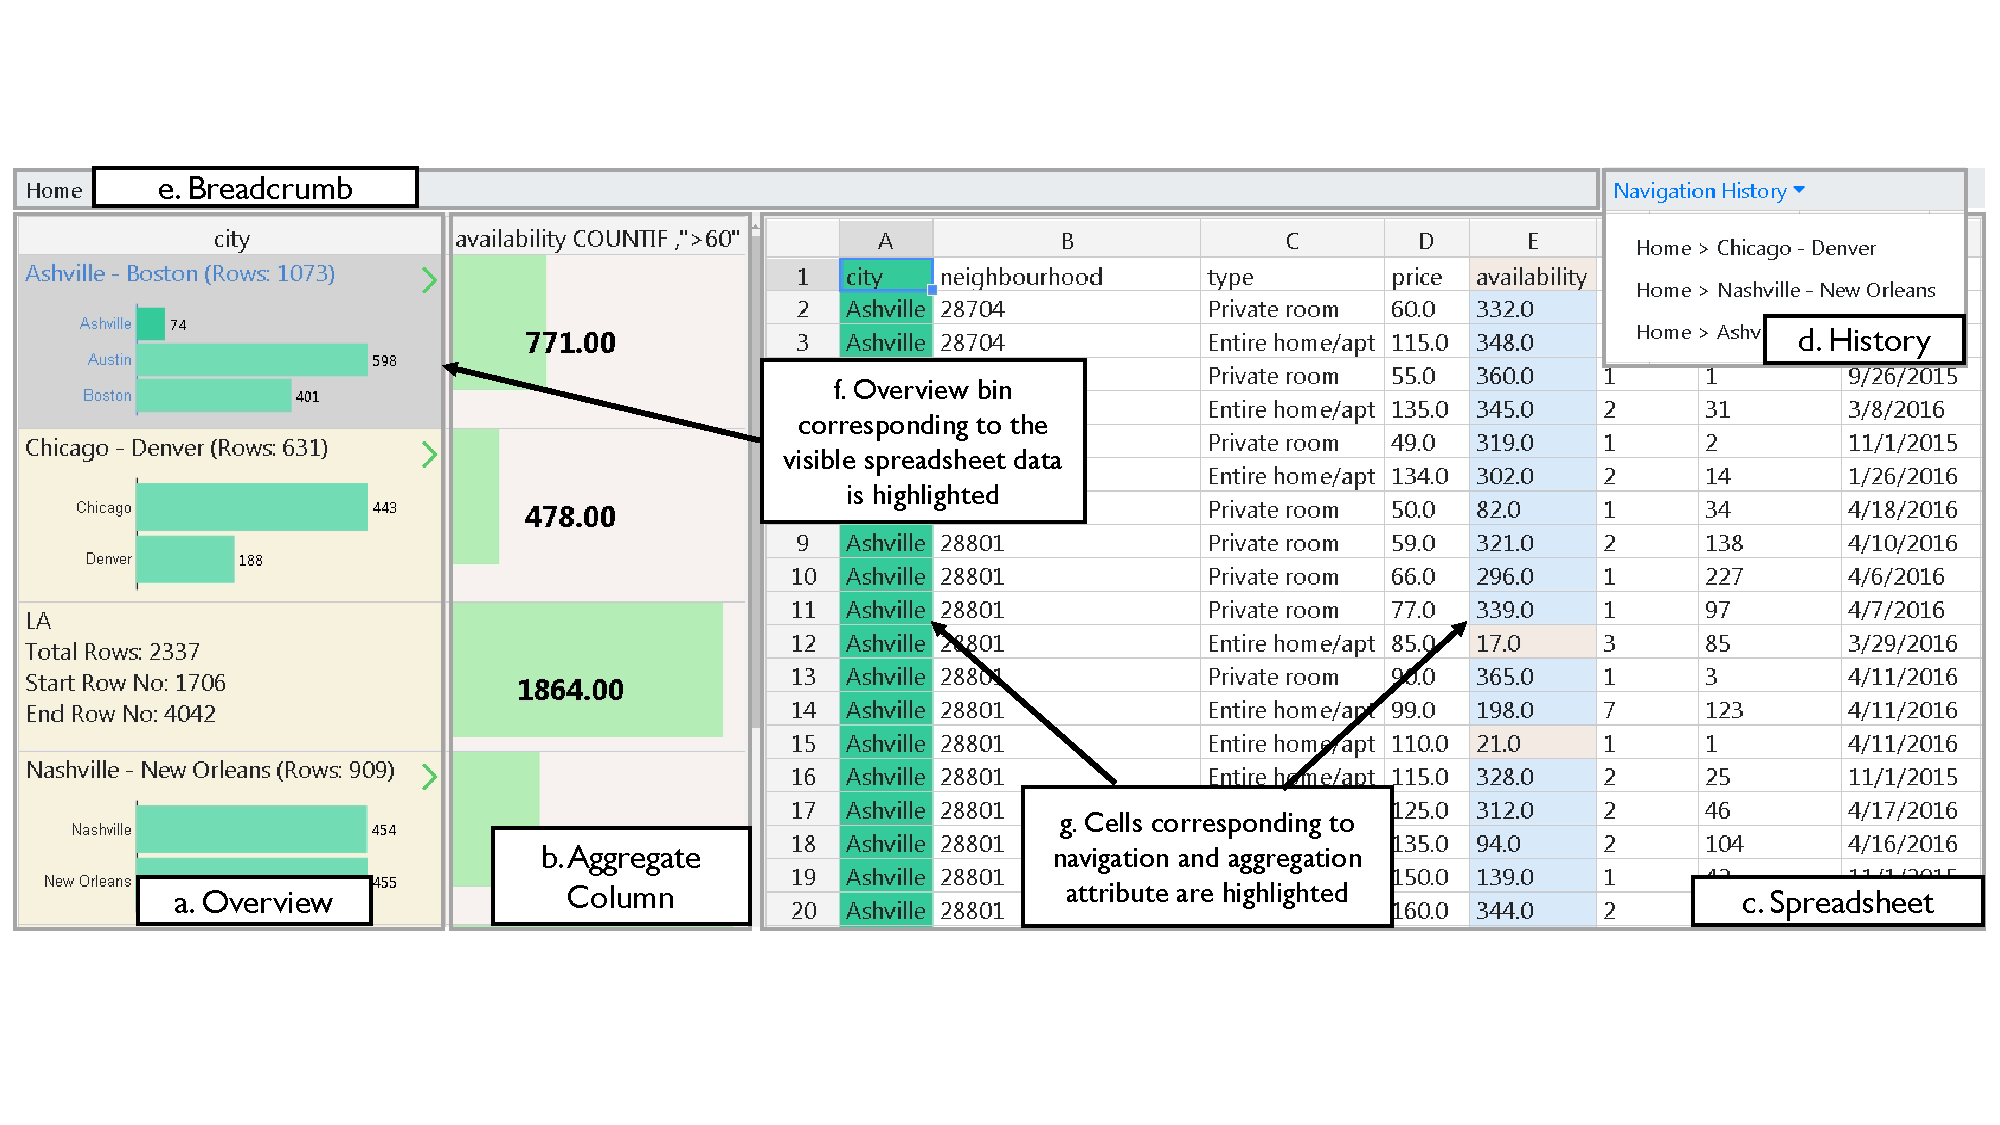
\includegraphics[width=\linewidth,trim={0 95 0 80},clip]{images/screenshot.pdf}
    \caption{\noah: navigation interface consisting of (a) a zoomable overview and (b) an aggregate column integrated with (c) a spreadsheet. A context bar consisting of (d) a navigation history displaying locations visited so far using the overview, and (e) a breadcrumb showing the current navigation path (\eg Home). (f) The user’s current focus in the spreadsheet is highlighted on the overview. (g) Columns corresponding to the navigation attribute (city) and aggregate column (availability) are highlighted on the spreadsheet.}
  \label{fig:ux}
\end{figure*}

\new{
However, navigating spreadsheets using scrolling or steering
is challenging, since spreadsheet data span multiple screens,
making it hard to synthesize, analyze, makes sense of, or
operate on it~\cite{network-context,nardi1990spreadsheet}.
With the ease of data generation, and with spreadsheets
now supporting increasingly larger datasets, \eg Google Sheets
now supports five million cells~\cite{gs}, a $12.5X$ increase
from the previous limit of 400K cells, 
{\em navigating
data within spreadsheets is only becoming even harder},
thanks to
multiple inter-related reasons: 
}
\squishlist
\item {\em Loss of overview and context.}
When navigating
spreadsheets, users can easily lose the context
of where they are and where they should go next~\cite{network-context}.
The only navigational context provided by spreadsheets
is the built-in scrollbar that acts as a one-dimensional
overview and indicates the user's current location on the sheet.
However, since this overview does not capture the
layout and structure of the data,
users are forced to mentally assimilate
the layout and recall it on-demand, as they navigate a spreadsheet.

\item {\em Cognitive and mechanical burdens.}
The lack of contextual cues leads to severe
cognitive and mechanical burdens
for users~\cite{cockburn2009review}.
Users often end up taking their own drastic measures to
avoid getting lost; for example,
some users create personalized overviews
extrinsic to the spreadsheet,
by sketching maps
of spreadsheets on paper~\cite{network-context}.
Other users add their own landmarks such as headers or
colored cells, as a visual affordance to assist
in navigation~\cite{network-context}.
Steering via dragging the mouse pointer across multiple screens to select
a subset of data as input to a formula
can often be challenging as well:
the only remedy is for users to abandon steering entirely and
instead remember the range of
the subset of data of interest, and then correctly enter this range
as the argument to the formula, often giving rise to errors that are increasingly prevalent in spreadsheets~\cite{panko1998we}.


\item {\em Visual discontinuities.}
The limited viewport afforded to the user
introduces a visual discontinuity between the
information being displayed.
For example, comparing spatially separated subsets
of data within the spreadsheet
requires moving back and forth between multiple viewports,
which can be overwhelming~\cite{nardi1990spreadsheet,network-context}.
As an alternative, users tend to copy subsets of data side by side to
reduce the visual discontinuity~\cite{nardi1990spreadsheet,network-context},
which is cumbersome.
\squishend

\noindent
Overall,  while navigating present-day spreadsheets, 
{\bf \em users often lose context,
get overwhelmed, and experience visual discontinuities.} 
Addressing these challenges requires considerable manual effort.
As we \new{will} argue in Section~\ref{sec:related},
existing spreadsheet features such as
pivot tables, named ranges, and subtotals,
\new{partially alleviate 
some of the aforementioned 
challenges but do not eliminate them entirely.
For example, pivot tables generate a summary
while losing the correspondence between the
raw data and the summary, while named ranges require users
to manually associate names with ranges of data.}


So, how do we support more effective navigation of data
within spreadsheets?
One approach would be to try to integrate
an overview of the overall structure of the data along
with the spreadsheet~\cite{grudin2001partitioning}
\new{resulting in} a classical
overview+detail interface
where the spreadsheet is the detailed view.
Overview+detail interfaces are used
to facilitate navigation in various domains such as 
text editors and maps~\cite{cockburn2009review}.
\new{Users can manipulate
the overview or detailed view,
to perform high-level or low-level operations,
respectively.}
Overview+detail interfaces
have been shown to be effective in these domains,
reducing cognitive load for users by
providing \new{them} the big picture first,
helping them quickly assimilate 
the information space~\cite{cockburn2009review}.
\new{Our goal is to {\em integrate an overview plug-in 
with spreadsheets} that captures
the overall structure of the data,
while supporting interactions that address
the difficulties in typical navigational 
operations like scrolling and steering.
{\bf \em It is essential
that our interface is a plug-in that 
enhances the capabilities of spreadsheets
that so many users
are used to and reliant on,
as opposed to a potentially jarring or confusing 
replacement for spreadsheets.}
}
% \saj{In this paper, our goal is to integrate an overview plug-in with spreadsheets that captures the overall structure of the data while allowing interactions that minimize the difficulties caused by typical navigational operations like scrolling and steering.}

However, while an overview plug-in for spreadsheets
does seem appealing and natural,
developing it leads to several challenges.

\squishlist
\item {\em Overview modality.}
\saj{
One approach for an overview is to simply add a
zoomed out version of the entire sheet as a pane on the side,
as in popular presentation software like 
Microsoft PowerPoint or text editors
like Sublime Text.
\newsaj{The zoomed out overview
displays the entire data 
at a lower magnification scale.} 
Unfortunately, this approach
would not suffice for a spreadsheet.
\new{An overview should provide a
comprehensible big picture view:
for a \newsaj{spreadsheet of numbers, text, or formulae}, 
when zooming out beyond a point, 
\newsaj{an overview displayed at 
such low magnification scale} 
would be unreadable.}
Another approach, adopted by map tools like the
early versions of Google maps,
is to use the overview
to provide a global context of the user's current location
being displayed in the zoomed in detailed view~\cite{cockburn2009review}.
While the overview remains static, users can perform semantic zooming operations~\cite{perlin1993pad} on the detailed
view which allows objects to be represented differently at different scales. Since spreadsheets already display the raw data,
zooming into and out of a detailed view consisting of
this raw data is not meaningful. 
\new{How do we design an overview to dynamically 
change as users 
seek a more fine-grained or coarse-grained view 
of the overall structure of the data?} 
}

\item {\em Construction of the overview.}
\saj{Given a spreadsheet
with many rows, 
one approach to constructing a dynamic overview 
is mapping rows of data to high level groups, 
similar to online maps. 
In online maps, cities are grouped into states 
and states are grouped into countries, 
forming a multi-granularity hierarchy. 
How do we automatically group spreadsheet 
rows together in a similar ``meaningful''
way
such that this grouping applies to all 
data types, including strings and numbers? 
If the automatically generated grouping is 
not semantically meaningful, how do we allow the users
to customize the grouping modality? 
How do we facilitate interactions that enable 
users to view the overview at multiple granularities?}

\item {\em Operations on the overview.}
\saj{Following the construction of a dynamic overview, 
the next challenge is to design simple interactions 
that achieve similar outcomes as scrolling and steering.
For example, an alternative to scrolling 
can be to leverage the groups of the overview 
to access the rows mapped to that group. 
\newsaj{As the granularity of the dynamic overview 
changes, how do we efficiently update the mapping 
from spreadsheet rows to the 
finer or coarser groups 
so that scrolling remains seamless? 
Similarly, how do we leverage
the overview to steer spreadsheet data (i.e., select a range of data)
for formula computation? How do we present the results of
the formula within the overview? One approach can be to adopt
the pivot table-like presentation of results. Within their summary view, 
pivot tables display 
aggregate formula results (\eg \code{SUM}, \code{COUNT}) 
alongside each group. 
However, unlike pivot tables, users can explore the overview at
multiple-granularities. As the granularity changes,
the grouping of rows also changes; 
making the previous formula results 
inconsistent with the new groups.
How do we 
recompute the results of a formula 
as the granularity changes 
without requiring the users to 
reissue the formula from scratch?}}
\agp{the last three questions are fairly confusing and assume that you already know what NOAH does.. can we simplify?}

\item {\em Seamless integration as a plug-in.}
\newsaj{Finally, how can we 
design an overview with a generic set of features,
that can be integrated
with any existing spreadsheet tool on any 
dataset without impacting
existing functionalities or look-and-feel?
How do we ensure that the interactions 
supported by the overview 
are 
consistent with
traditional spreadsheet semantics,
and complement existing spreadsheet interactions?
How to we enable coordinated interactions across both views, \ie 
the overview and the raw spreadsheet, such that they
remain consistent at any given time?}
\squishend
\agp{A general comment: can we ensure that either we use
questions for all of the items above or none of them for uniformity?}

\stitle{\noah: \new{a navigation plug-in for spreadsheets}.} We address the aforementioned challenges
in \noah,
an in-situ
\textbf{\underline{n}}avigation interface
for \textbf{\underline{o}}verviewing
and \textbf{\underline{a}}nalyzing
spreadsheet data \textbf{\underline{h}}olistically.
\noah is constructed as a plugin to
an existing spreadsheet tool,
{\scshape DataSpread}~\cite{dataspread},
an open-source scalable web-based spreadsheet.
While \noah's design is not tied to {\sc DataSpread},
we opted not to use other popular spreadsheet
tools like Google Sheets and Microsoft Excel because they
are closed source.
Figure~\ref{fig:ux} shows a snapshot of \noah.
When the user chooses to explore
the data by a specific attribute,
\saj{a multi-granularity overview is constructed and displayed
within \noah, next to the raw spreadsheet data (Figure~\ref{fig:ux}a). Users can zoom into or out of the overview to obtain a \new{fine or coarse-}grained 
perspective of the data distribution. 
The distribution at each granularity 
is captured by a histogram,
enabling users to assimilate the data \new{via summary
statistics}. 
Each bin (group) of the histogram is 
mapped to a collection of rows in the spreadsheet.} 
Cumbersome scrolling operations are eliminated in favor
of a few clicks on the overview interface. Instead of steering to analyze the data,
users can issue formulae
on the overview with interactions similar to pivot table construction,
and view results on a separate {\em aggregate column},
alongside the overview (Figure~\ref{fig:ux}b). 
In this manner,
users can issue formulae on different
subsets of the data while remaining on the same screen,
reducing visual discontinuity.
\noah ensures that there is coordination between
the overview and the spreadsheet:
for example, panning and zooming on the overview
are reflected on the spreadsheet by displaying
the spreadsheet data corresponding to the bin
currently in focus in the overview.
Finally, \noah automatically creates
contextual and historical information
(Figure~\ref{fig:ux}d and~\ref{fig:ux}e)
while displaying visual cues
(Figure~\ref{fig:ux}f and~\ref{fig:ux}g)
so that users don't lose context during navigation.

The primary contribution of our work is twofold:
\squishlist
\item We formalize the design of a general
navigation (overview+detail) interface
for exploration and analysis of large spreadsheets.
We realize this design in the form of \noah,
a plugin to an existing web-based spreadsheet tool,
ensuring that interactions supported by \noah
complement existing spreadsheet operations.
\item We conduct a user study to evaluate
the benefits and limitations of this plugin.
\newsaj{The study required users to
perform tasks that were representative of
popular spreadsheet operations,
using both Microsoft Excel and \noah.}
\saj{The study shows that compared to Microsoft Excel, participants were able to complete spreadsheet
tasks involving navigation 
correctly and quickly in \noah. Participants made {\bf $2.5\times$ fewer} mistakes while being {\bf $2\times$ faster} with a \noah-integrated spreadsheet than with Excel.} \agp{mention how these tasks were representative or general}
\squishend


\toappendix{The rest of the paper is organized as follows: In Section~\ref{sec:usage} we first present a case study of \noah being applied to a real-world scenario.  
In Section~\ref{sec:related}, we discuss related work. We then explain the design considerations for developing \noah in Section~\ref{sec:design}. In Section~\ref{sec:ui}, we present \noah’s user interface and supported operations. We then discuss the design and outcomes of a user study evaluating the effectiveness of \noah in Section~\ref{sec:study}. Finally, we discuss the limitations of \noah and possible future enhancements in Section~\ref{sec:discuss}.}


%!TEX root = main.tex

\section{Related Work}
\label{sec:related}
We now discuss tools and techniques
that partially address the limitations of navigating
spreadsheets.

\subsection{Spreadsheet Tools and Prototypes}
\cut{Commercial spreadsheet tools include
Microsoft Excel, Google Sheets, and Airtable---of
these, Excel and Google Sheets support features
targeted at improving users' navigation experience.}
\agp{Abrupt, add at least one line to say that existing spreadsheet tools recognize challenges in nav or something}
\newsaj{Existing spreadsheet tools---both commercial software and academic prototypes---recognize some of these navigation challenges while adopting different measures to address those.}

\cut{Excel allows users to maintain context during navigation
by manually creating named ranges~\cite{named-range},
that are essentially references
to a spreadsheet region,
and appear in a \emph{name box}
within the Excel menu bar.
Users can click on a named range
to navigate to the referred region.
However, the onus is on the user to create
named ranges for each region of interest.}
\stitle{Microsoft Excel.}
\new{Excel enables users to manually create references
to a spreadsheet region using the named 
ranges~\cite{named-range} feature,
accessible from the menu bar.
Users can click on a named range
to navigate to the referred region. 
However, the onus is on the user to create
named ranges for each region of interest. 
The pivot table~\cite{pivot} feature 
allows users to create a summary view to 
compare subsets of data without having to 
provides a summary view, enabling users
to compare subsets of data without
having to navigate to various locations
within the sheet.
This summary is placed
in a separate region of the spreadsheet,
preventing users from accessing
the data underlying the summary, impeding navigation. 
A similar overview feature, \code{SUBTOTAL}~\cite{subtotal},
adds a new row at the end of each distinct
subset of data with summary
information. Users can expand the summary to view
the actual spreadsheet data.
However, for datasets with many subsets (\eg for numeric data),
the number of new lines inserted (i.e., the summary) 
can itself become very
large, spanning multiple screens, and can cause
increased
visual discontinuity during navigation. Finally, NodeXL~\cite{hansen2010analyzing}
is a plug-in that provides a spreadsheet network overview
and supports navigational operations,
\eg zooming in/out, dynamic filtering, on the overview;
this plug-in only supports network datasets,
such as biological or social networks.}

\stitle{Google Sheets Explore.}
Google Sheets Explore~\cite{web:explore} provides
an overview of the data by
auto-generating charts of data statistics.
Users can specify queries to the system
(similar to a web search)
asking for different summary statistics.
While Explore
is a convenient means to understand
high-level data characteristics,
it doesn't address the
navigational challenges
related to scrolling and steering.  
 
%\subsection{Academic Spreadsheet Prototypes}
\cut{Existing academic work focuses
on adding a richer set of operations to spreadsheets,
or increasing their scalability.
We discuss work specifically targeting
navigation; other enhancements
such as managing hierarchical data~\cite{chang2016using}
or supporting joins~\cite{bakke2011spreadsheet},
are omitted.}

\stitle{Scalable Spreadsheet Summarization and Exploration.}
Smart-drill-down~\cite{joglekar2015smart}
generates an interactive summary of a large spreadsheet table as
a collection of rules; users can drill-down to
a specific rule to view more fine-grained rules.
Hillview~\cite{web:hillview} displays
the approximate results of group-by queries
on large spreadsheet tables.
While these tools support summarization at scale,
providing an overview of the spreadsheet,
they don't preserve spreadsheet semantics,
nor do they make it easy to scroll or steer
through large spreadsheets.
ABC~\cite{Raman99scalablespreadsheets} and {\sc DataSpread}~\cite{datamodels} support interactive
exploration of very large spreadsheet datasets,
beyond main-memory limits, maintaining spreadsheet look-and-feel,
but do not provide any new spreadsheet capabilities to assist
with navigation.
We build \noah as a plugin
to {\sc DataSpread}, since it is open-source.

\stitle{Interactive Tables.}
TableLens~\cite{rao1994table}
is a focus+context view
for browsing numerical information
in tables, looking
much like a spreadsheet with embedded bar charts.
Cells out of focus display
graphical bars proportional in length
to the underlying values,
providing a visual overview of the data,
while cells within the user's current focus
are magnified and display the graphical bars and
the raw data.
Ideas similar to TableLens
have been adopted by DataLens~\cite{bederson2004datelens}
for visualizing digital calendars, and
by FOCUS~\cite{spenke1996focus}
and InfoZoom~\cite{spenke2003visualization}
for exploring database query results.
Like TableLens, \noah
embeds graphical bars, but within
the overview to depict the underlying data
distribution. \noah captures
the user's current focus by highlighting
the corresponding bin in the overview.
While TableLens provides an easy mechanism
to get a high-level view of the data
and spot outliers, it
suffers from the same disadvantages
that focus+context views have relative
to overview+detail ones.
Unlike \noah, which supports
multiple granularities via binning,
TableLens only supports
one granularity (zoomed in or
zoomed out): beyond
a certain size, navigating (scrolling or steering)
the zoomed out data
is still cumbersome for users. Moreover, TableLens does not maintain the spreadsheet look-and-feel or capabilities.
%TableLens does not support non-numeric data,
%nor does it maintain the spreadsheet look-and-feel or capabilities
%(maintained in \noah due
%to the detailed view).


\stitle{Visual Interactive Spreadsheets.}
VisSh~\cite{nunez2000vissh}, SI~\cite{levoy1994spreadsheets},
SSR~\cite{chi1997spreadsheet}, ASP~\cite{piersol1986object},
and PhotoSpread~\cite{kandel2008photospread}
extend the input/output capabilities of cells
within spreadsheets, to
display charts, animation, photos, or geometric objects, or
accept input via direct manipulation dialogs,
among others.
While these tools allow users to represent and manipulate
data in a more flexible manner,
which in turn could help users getting a
high-level sense of the data,
they do not necessarily help users navigate data
more effectively.





\subsection{Spreadsheet Alternatives}
%Finally, we discuss solutions to navigational and summarization
%challenges in other domains.

\stitle{Overview+Detail Interfaces.}
Cockburn et al.~\cite{cockburn2009review}
provides a detailed survey of overview+detail
and zooming interfaces.
To improve navigation within large documents,
overview+detail interfaces~\cite{cockburn2006faster,kratz2010semi} allow users to interact with an overview as they explore the document. Zooming interfaces~\cite{nekrasovski2006evaluation,plaisant2002spacetree} provide a multi-granularity overview of the data and support interactions like zoom in/out to navigate across various granularities.
We follow the same analogy of
providing an overview of the spreadsheet first,
allowing users to drill-down further.

\stitle{Multiple Coordinated Views.} Multiple coordinated views~\cite{roberts2007state}, \eg \emph{Snap}~\cite{north2000snap}, \emph{Elastic Documents}~\cite{badam2018elastic} connect multiple views, for example, an overview and a detailed data view while enabling coordination between these views through brushing and linking. Similarly, \noah connects tabular spreadsheets with an overview and updates the state of the spreadsheet as users interact with the overview and vice-versa.

\stitle{Tabular Data Analysis (TDA).}
Visualization tools such as Tableu~\cite{tableau}, Power BI~\cite{powerbi}, Keshif~\cite{yalccin2018keshif}, Voyager~\cite{wongsuphasawat2016voyager} and
analytical tools such as SPSS~\cite{noruvsis1986spss}, SAS~\cite{sas1985sas}, can all provide summaries of tabular data in various forms (visualizations,
aggregate statistics). 
\new{These summaries 
are static overviews of the data---much like pivot tables, 
these summaries are not dynamically linked
to nor are co-located with
the underlying raw data. \newsaj{For example, Keshif~\cite{yalccin2018keshif} can display all the unique values corresponding to an attribute of interest, \eg cities of the Airbnb data~\cite{web:airbnb}. However, users cannot view or inspect the raw data corresponding to each city. With TDA tools, the spreadsheet look-and-feel is lost,
and as a result, users
loose the capability to directly manipulate raw data, derive new data, and issue formulae for free-form analysis.}  
\cut{For example, using these tools users cannot \code{browse} subsets of data and \code{lookup} or \code{locate} data points of interest (see Table~\ref{tab:scope}). Aditya: previous line problematic: they can... because all these tools support to varying extents the typology. Even users of such tools want to inspect the underlying data to verify the summary statistics and visualizations~\cite{2017trust}. Aditya:this line is problematic too... because the citation is to an AQP tool rather than some general purpose study}
\newsaj{Therefore, the goals of spreadsheets differ from TDA 
tools in two ways: a) facilitating direct manipulation of raw 
data and b) enabling arbitrary derivation of new data and summaries
using various operations involving navigation,
\eg formulas or expressions.}
\noah being a plug-in to spreadsheets, 
facilitates a unified interface that
upholds both these goals
while enhancing
navigational capabilities
for spreadsheet users.
}
\section{\noah: Design Considerations}
\label{sec:design}
In this section,
we outline our design considerations
for a spreadsheet navigation interface.
%In our supplementary material,
%we additionally characterize
%the use-cases that such a navigation %interface
%is good for and not good for.
Our design considerations were
informed by prior work on
information visualization~\cite{shneiderman2003eyes,brehmer2013multi}, overview+detail interfaces~\cite{cockburn2009review}, multiple-coordinated views~\cite{wang2000guidelines},
and refined through our experiences
across multiple design iterations.

\para{DC1. Construct the overview in-situ}
An overview helps users get a high-level picture
of the data.
However, maintaining the overview in a separate
location from the data can \newsaj{lead to loss of context};
instead, having it co-located with the data
can help users make rapid glances to
explore information between a
bird's-eye view
and a close-up detail~\cite{grudin2001partitioning}.

\para{DC2. Ensure reduced
visual discontinuity while providing details on demand}
Users often need to access subsets of data,
and study their properties in detail, \eg via steering.
Navigating back and forth \saj{between different subsets of data}
can lead to increased visual discontinuity.
The interface should allow users to compute such details for
various data subsets on demand~\cite{shneiderman2003eyes}.
The interface should maintain visual continuity
as users navigate to a different subset,
recomputing the details for the new subset.

\para{DC3. Balance the screen space afforded to the overview}
As the overview
has limited screen-space available,
we need to consider the trade-off between visual discontinuity (\emph{DC2}) and clarity.
\saj{Displaying a fine-grained overview improves visual clarity while increasing visual discontinuity---users need to scroll through the overview to access distant
subsets of data.
Displaying a coarse-grained overview decreases visual discontinuity at cost of reduced visual clarity---the overview may span too many data subsets and appear visually cluttered}.
The interface should further allow users to control the screen-space allocated
to the overview.


\para{DC4. Enable coordination between the spreadsheet and overview}
Since users can view the overview
and the spreadsheet simultaneously,
interactions on both need to be linked~\cite{roberts2007state},
\ie an interaction on one should be reflected on
the other~\cite{wang2000guidelines}.
For example, as a user scrolls through
the spreadsheet, the user's current focus
should be highlighted on the overview.
However, not all interactions need to be interlinked,
\eg changing the font size of a spreadsheet cell
need not lead to a change in the overview.



\para{DC5. Facilitate customization of the overview}
As the overview is automatically generated,
it may not reflect domain-specific context
known only to the user~\cite{Raman99scalablespreadsheets}.
For example, an overview constructed on a grading
spreadsheet by binning nearby scores
may not match the letter grade ranges
that the instructors have in mind.
Allowing users to customize the overview is therefore essential.

\para{DC6. Display contextual and historical navigation information}
The interface should record navigation history,
allowing users to revisit previously visited locations~\cite{shneiderman2003eyes},
while also displaying their current navigation path for context.

\section{User Interface}
\label{sec:ui}
We now explain the design of \noah's components
and implementation details.

\subsection{In-situ Overview}

\noah constructs the overview in-situ ({\bf DC1})
next to the spreadsheet
on an attribute of the spreadsheet dataset
called the {\em navigation attribute},
selected by the user.
Any attribute type that can be ordered
can be a navigation attribute, \eg
text, numbers.
The overview is constructed at multiple granularities.
Each granularity is divided into non-overlapping
groups of data called {\em bins}.
As shown in Figure~\ref{fig:concept}d,
an overview of the Airbnb data
on the navigation attribute ``city''
has granularity levels.
The highest (coarsest) granularity level
consists of four bins.
Figure~\ref{fig:concept}a
depicts the first four bins,
the first of which is {\em Ashville-Boston}.
Each bin contains summary information
regarding the data subset/region
it spans, \eg starting row and
ending row number, and 
the total number of rows the region spans.
Each bin displays an overview
of the next (finer) granularity (if any)
with embedded bar charts.
For example, in Figure~\ref{fig:concept}d,
the topmost bin ({\em Ash-Bos}) spans three cities
({\em Ashville}, {\em Austin}, {\em Boston}), each of which is a bin
in the next (finer) granularity.
Correspondingly, Figure~\ref{fig:concept}(a)
shows three horizontal bar charts for the
first {\em Ash-Bos} bin,
one for each bin in the next granularity.
Since the third bin from the top
(\emph{LA}) spans only one city,
no bar chart is embedded.
Users can perform different
operations on the bins, \eg clicking to pan and
semantic zooming in/out~\cite{perlin1993pad}.
\noah supports other interactions,
\eg customization and aggregation.
We discuss these interactions
in the context of our design considerations in Section~\ref{sec:overview_operations}.

\stitle{Why a Multi-granularity Binned Overview?}
\saj{A standard overview approach
is to show a spatially partitioned
collection of thumbnails \saj{on the left of the detailed view},
similar to Microsoft PowerPoint or
Adobe Reader.
However, displaying too many thumbnails
results in increased scrolling
to access distant thumbnails,
increasing visual discontinuity.
On the other hand,
displaying too few thumbnails
reduces visual discontinuity,
but at the cost of visual
clarity---the thumbnails appear cluttered
and fail to represent the
underlying data clearly~\cite{cockburn2009review}.
To strike a balance between these two objectives
({\bf DC3}) we designed a multi-granularity overview
that abstracts the data at varying levels of detail.
Multi-granularity interfaces
provide an alternative to \newsaj{the spatially partitioned single-granularity representation of the data space, \eg in Powerpoint, by allowing users to control the scale at which the overview should be displayed~\cite{cockburn2009review}.}
Users can resize the overview to control the amount of spreadsheet data that remains visible.
\toappendix{Microsoft PowerPoint also uses a
similar technique to balance the screen
space between overview and detail.}
Users can also hide the overview if required.}

\newsaj{The data structure underlying the overview
is an equi-depth histogram constructed
on the values
in the navigation attribute column.
Equi-depth histograms are commonly
used for summarizing the statistical properties
of data, with applications such as
database query optimizers~\cite{chaudhuri1998random}.
The binned representation of the overview
using equi-depth histograms
enables faster navigation
by reducing visual discontinuity. 
The bins act as landmarks
in the overview, enabling 
users to skip irrelevant bins
and quickly navigate to the desired subset of data. We now discuss how the overview is constructed.}


\stitle{Overview Construction.}
\newsaj{The equi-depth histogram 
can be constructed on 
any data types
that can be ordered, \eg text, numbers, dates. For example, 
in the usage scenario explained in Section~\ref{sec:usage},
the journalist grouped the data into cities
for ease of navigation 
when exploring the larger cities
in the Airbnb dataset.}
Each bin in the equi-depth histogram
contains the same number of items,
where each item is a value.
For example,
when constructing the overview
on city,
each value in the city column
is assigned to a bin.
The bins are constructed top-down
(see Figure~\ref{fig:concept}d). \noah divides
each of the bins at level $k$ into new bins
to construct the next lower level $k+1$, again,
by applying the same concept of equi-depth histograms.
If each value of the navigation attribute
column was unique, \eg if it was a numerical ID,
then construction of the histogram would be easy:
each bin of the equi-depth histogram
would contain almost the same number of items,
where each item corresponds to one unique value of
the attribute.
Unfortunately, in practice, for many attributes,
the same value is often repeated.
For example,
there are multiple listings
per city.
Therefore,
an equi-depth histogram
on the
attribute city
will result in consecutive bins
sharing items of
the same unique city value,
resulting in undesirable overlap.
Instead,
we construct a best effort
equi-depth
histogram that is as close to an equi-depth
histogram as possible, while ensuring
that the ranges represented by each bin have no overlap.
\agp{Aditya: would be valuable to describe the algorithm to increase
technical depth.}
\saj{Saj: can we add a pseudocode in appendix and refer to that?}


\begin{figure}[t]
        \centering
        %\vspace{-10pt} %trim=left bottom right top
        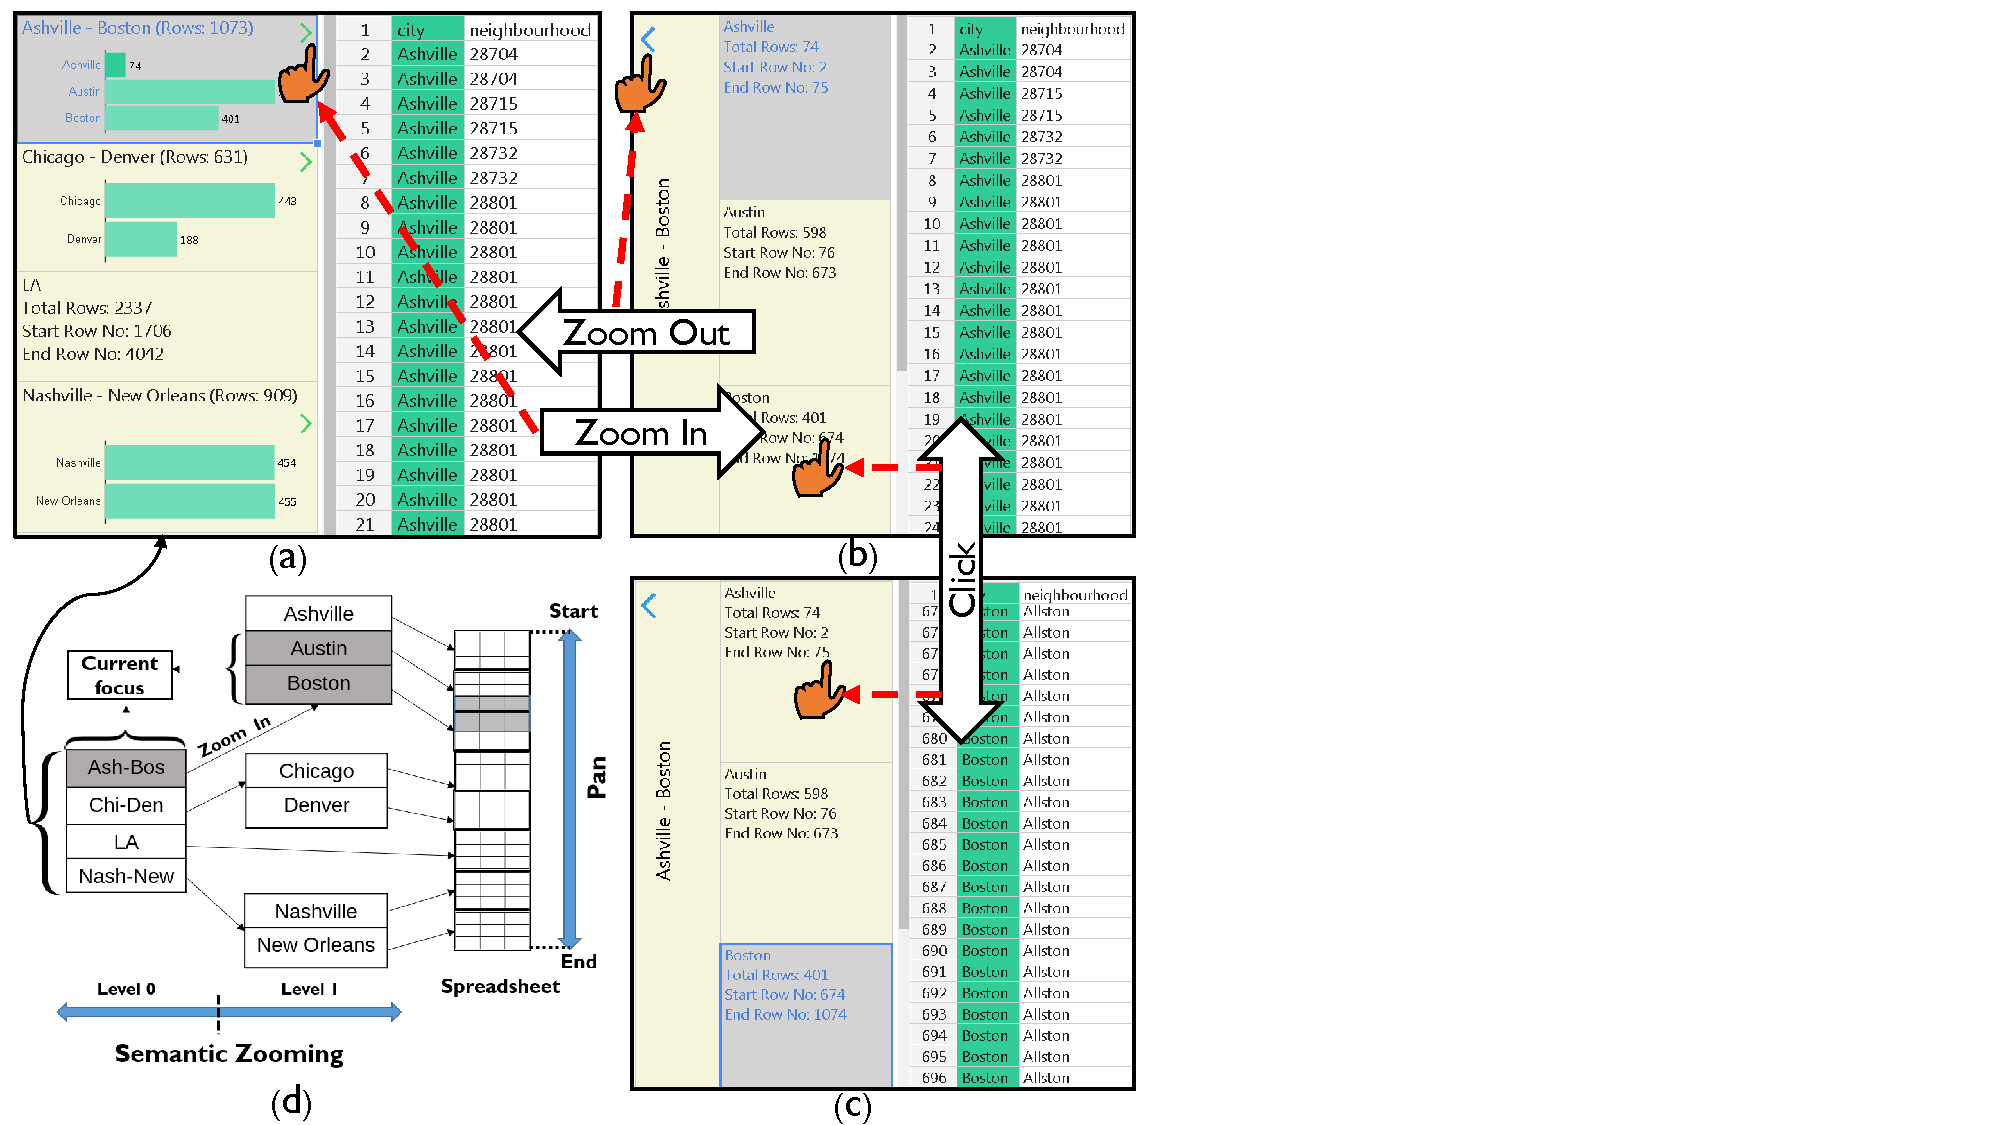
\includegraphics[width=0.45\textwidth,trim={0 0 400 0},clip]{images/navigationOp.pdf}
\vspace{-10pt}
   \caption{Navigational operations. (a) The overview at the highest level of granularity. (b) A zoomed in view of the \emph{Ashville-Boston} bin. (c) As the user clicks on the \emph{Boston} bin, the Boston listings are displayed on the sheet. The \emph{Boston} bin is highlighted in gray to indicate user’s current focus. (d) Conceptualizing the multi-granularity overview. }
\vspace{-18pt}
   \label{fig:concept}
 \end{figure}

\subsubsection{Operations and Interactions}
\label{sec:overview_operations}
We now discuss the operations and interactions that can be performed on the overview.

\stitle{Navigational Operation: Clicking.}
When a user clicks on a specific bin,
\noah displays the corresponding spreadsheet data;
users can use this to jump to a specific spreadsheet location
without having to scroll endlessly.
For example, in Figure~\ref{fig:concept}b,
as the user clicks on the \emph{Boston} bin,
the data corresponding to Boston is displayed
(Figure~\ref{fig:concept}c).
Note that the click operation is different from the traditional
spreadsheet \code{Filter} operation.
\code{Filter} hides spreadsheet data
that do not satisfy the filtering condition while
clicking brings the desired subset of data
in view without hiding the rest.
Users are free to navigate to other portions
through scrolling
even after clicking a bin, unlike filtering,
where users need to issue another \code{Filter}
to bring other data into view.


\stitle{Navigational Operation: Semantic Zooming.}  
Users can zoom into a specific bin
to view more fine-grained information or zoom out
to view more coarse-grained information,
via semantic zooming~\cite{perlin1993pad}.
For example, in Figure~\ref{fig:concept}a,
from the bin \emph{Ashville-Boston}
when the user zooms in to the next level,
\noah displays the bins \emph{Ashville}, \emph{Austin},
and \emph{Boston} (Figure~\ref{fig:concept}b).
If the user zooms out of the current granularity, again \noah displays the bins \emph{Ashville-Boston}, \emph{Chicago-Denver}, and others.
Users can only zoom into any bin that
contains multiple unique values.
For example, in Figure~\ref{fig:concept}d, at level 2,
each bin corresponds to one city.
Therefore, users can only click on those bins
to bring that data into view, and cannot zoom in further.
One issue with zooming interactions
is discoverability \saj{of the zoom operation}~\cite{cockburn2009review}.
We circumvent this (see Figure~\ref{fig:concept}c)
by providing the root of the bin under selection
for zoom out, and arrows for
clicking to zoom in (``\textcolor{blue}{$\rangle$}'') and out (``\textcolor{blue}{$\langle$}'').

\stitle{Customizing the Overview.}
As \noah constructs the overview automatically,
the overview binning or organization
may not capture domain-specific context
or user needs.
\noah enables users to customize\toappendix{ (\code{create} in Table~\ref{tab:scope})} this organization (\textbf{DC5}).
At any granularity, users can merge multiple consecutive bins
into a single bin, or split a bin into multiple bins.
\toappendix{The other operations include merging all the bins into one single bin and collapsing all the bins into singular bins, \ie one unique value per bin.}
Say the user wants to compare summary statistics
of Boston and Chicago.
In the current organization
these two cities are  
in two different bins (see Figure~\ref{fig:customize}a).
Using the bin customization feature,
the user can merge the two bins
\emph{Ashville-Boston} and \emph{Chicago-Denver} to create a new bin \emph{Ashville-Denver}.
Users can now zoom into this bin and
compare summary statistics of the cities in the same view.
The interactions for splitting a
bin depend on the data type.
If the navigation attribute is textual,
any bin can be split into as many bins as the
number of unique values that bin contains.
If the navigation attribute is numeric,
users can split the bin into any arbitrary number of bins.
Note that \noah does not allow users to rearrange the
order of the bins.\toappendix{ Users can only customize the boundary of the bins.} Since the overview represents a histogram, the bins are ordered---reshuffling the bins violates that order.

\begin{figure}[!htb]
        \centering
        \vspace{-8pt}
        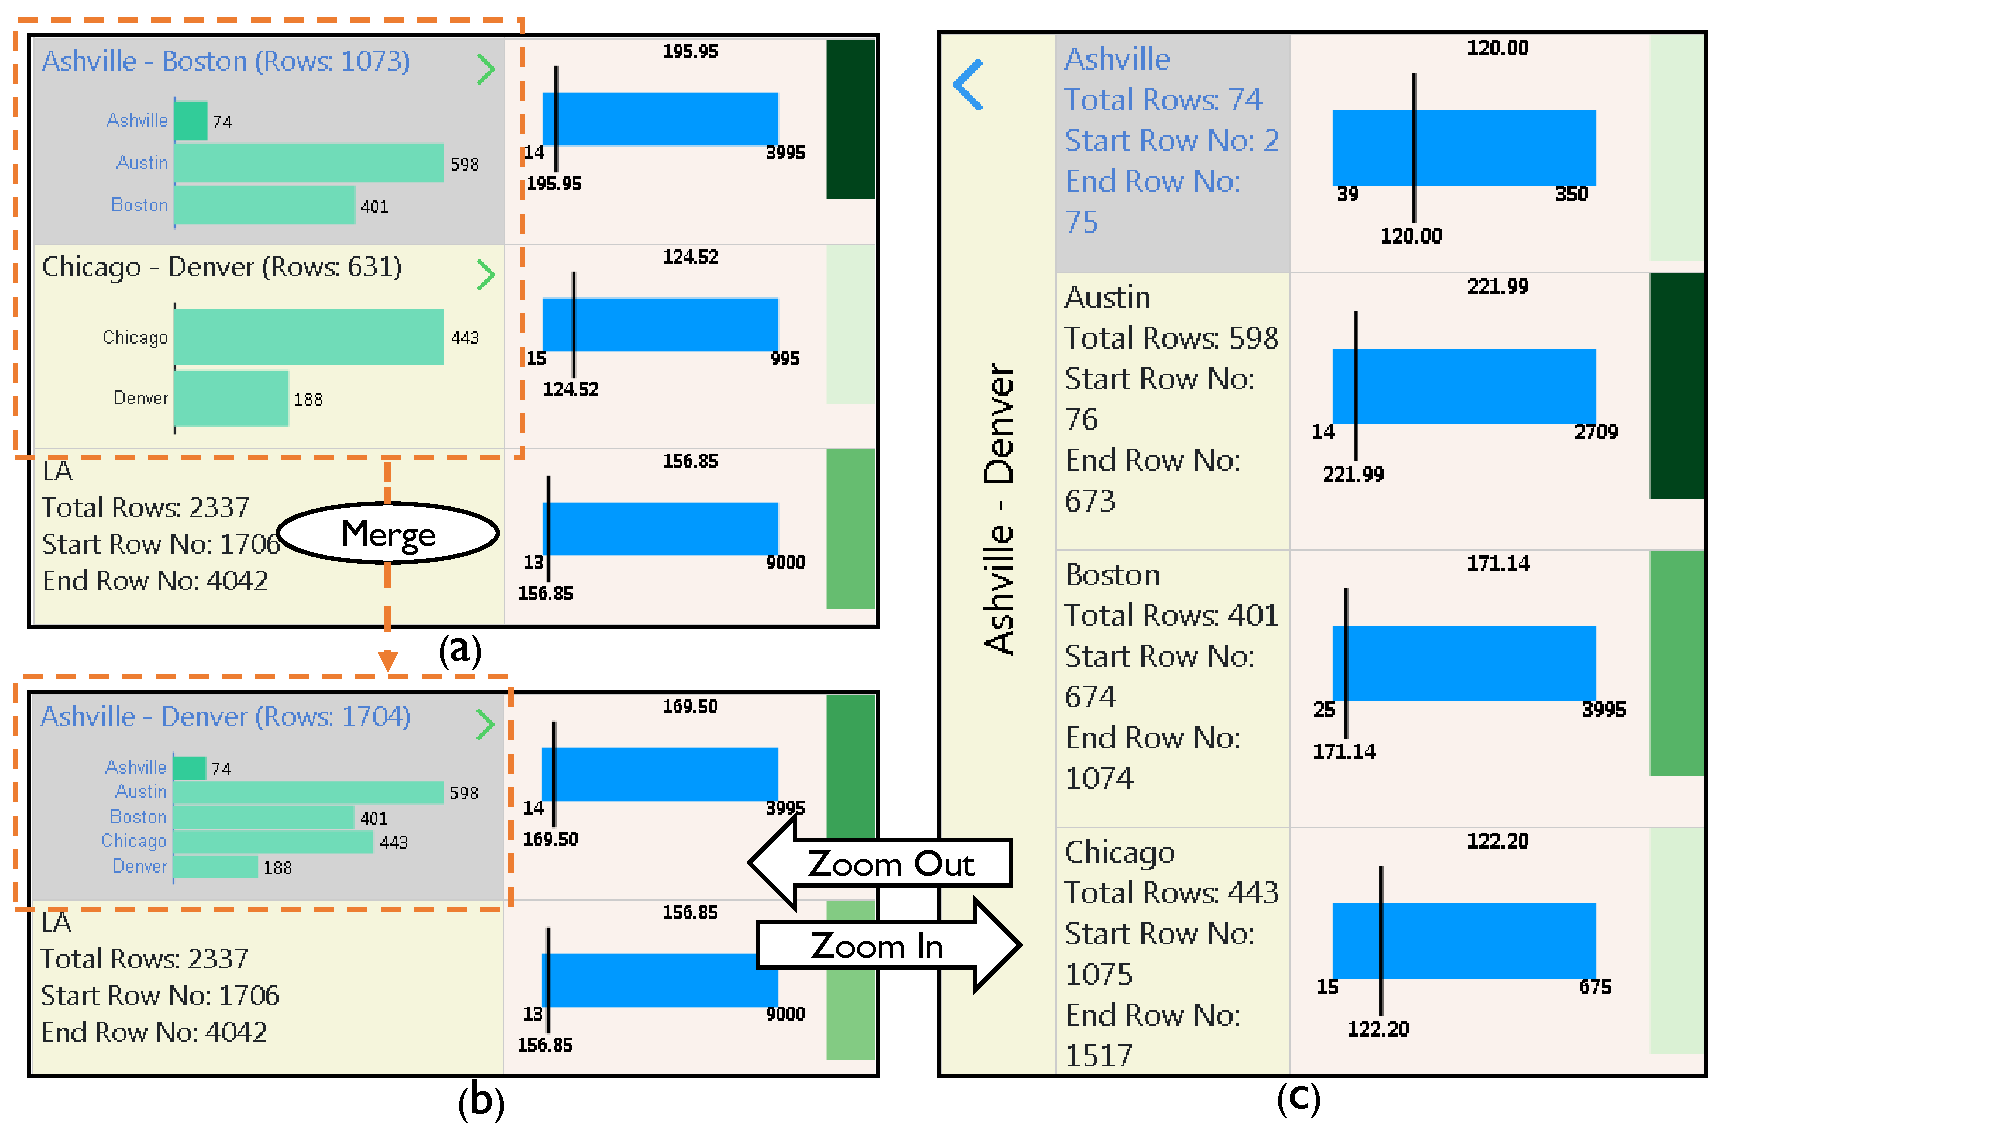
\includegraphics[width=0.45\textwidth,trim={0 0 130 0},clip]{images/customize.pdf}
\vspace{-10pt}
   \caption{(a) Chart view of the aggregate column. (b) A new bin is created by merging the top two bins. (c) Zooming into the newly created bin. }
\vspace{-10pt}
   \label{fig:customize}
 \end{figure}

\subsubsection{Coordination Between Overview and Spreadsheet}
\noah supports coordination
between the overview and the
corresponding spreadsheet data (\textbf{DC4}),
\ie interactions on the overview
may be reflected on the spreadsheet and vice-versa.
\newsaj{One example of this coordinations is,} indicating the navigation attribute on the spreadsheet
using color (see the lime green column in Figure~\ref{fig:ux}c)
as user constructs the overview. However, not all overview interactions are coupled
with the spreadsheet and vice versa.
The coupling depends on the user's current
focus---\emph{\saj{to ensure consistency between the overview and the spreadsheet,} any interaction on
either interface
that changes the current focus must be reflected
on the other interface}.
We now provide examples of both
coupled and decoupled interactions.

\stitle{Coupled interactions.}
Clicking a bin is an example of a coupled interaction
as the user actively changes the focus
to another bin on the overview.
To reflect the change, \noah populates
the corresponding spreadsheet data
on the screen.
As the user scrolls on the spreadsheet,
again the current focus changes
and the corresponding bin on the overview is highlighted.
For example, in Figure~\ref{fig:concept}c,
as the user clicks on the Boston bin,
the spreadsheet displays the Boston listings.
Conversely, as the user scrolls up,
both Austin and Boston listings appear in the current window of the spreadsheet.
Therefore, both the Austin and Boston overview
bins are highlighted
(see Figure~\ref{fig:concept}d).
%The zoom in operation, on the other hand,
%can be either coupled or decoupled based on the setting.
%Whenever a user zooms into a bin
%that is not the current focus,
%the spreadsheet is updated to show data
%for that bin.

\stitle{Decoupled interactions.}
When a user zooms into a bin
that is already in the user's current focus,
the spreadsheet view does not change.
For example, in Figure~\ref{fig:concept}a,
the user zooms into the \emph{Ashville-Boston} bin;
here, the spreadsheet view stays the same
(see Figure~\ref{fig:concept}b).
Similarly, the zoom out operation is decoupled.
When a user zooms out,
the overview displays
a coarser granularity view
of the user's current focus.
Since the focus stays the same,
there's no need to update the spreadsheet view.
Similarly, operations like panning on the overview without clicking,
and customizing the overview
do not change user's current focus and are therefore decoupled.
Online maps also adopt similar
decoupling of the overview and detail~\cite{cockburn2009review}.
However, their goal is to reduce network
and computational overload, whereas in our case,
the decoupling is based on the user's current focus.

\subsection{Aggregate Columns}
Users can issue spreadsheet formulae
on the overview
to compute aggregates for the data
in each bin\toappendix{ (\code{summarize} in Table~\ref{tab:scope})}.
The results
are displayed as an {\em aggregate column} (see Figure~\ref{fig:ux}b). Each entry in the aggregate column
corresponds to the adjacent bin
in the current granularity
of the overview.
For example, in Figure~\ref{fig:customize}c,
the aggregate column displays
four aggregate statistics,
one per bin.
Users can issue several formulae simultaneously,
each giving rise to a new aggregate column.
However, adding an aggregate column
takes up screen space, shrinking the spreadsheet view.
As a workaround, users can resize or
remove aggregate columns if required (\textbf{DC3}).
When the user issues a formula on the overview,
the spreadsheet column
corresponding to the aggregate column
is highlighted in grayish orange
(see Figure~\ref{fig:ux}c)---another example of coupled interaction.
For conditional formulae like \code{COUNTIF},
cells that satisfy the condition
are highlighted, \eg in Figure~\ref{fig:ux}c,
the cells with availability $\ge 60$ are colored in sky blue.
In this manner,
users can quickly determine which cells
are relevant to the aggregation operation\toappendix{ (\code{identify} in Table~\ref{tab:scope})}.

Creating an aggregate column on the overview mimics how users create pivot tables. Users
are not required to explicitly type formulae;
rather they simply select the formula from a drop-down menu,
and provide the necessary formula parameters to a form.
\newsaj{The aggregate column can employ any} statistical
and mathematical formulae that
operate over a range of data.
\newsaj{Therefore, creating an aggregate column
is equivalent to selecting subsets of data
on the sheet, \ie steering, and then executing a formula on this subset},
helping users avoid cumbersome steering operations.
We have classified the formulae supported
into five categories: a) summary (\eg min, max, average),
b) frequency (\eg mode, large, small), c) conditional (\eg countif, sumif), d) spread (\eg var,stdev), and e) others (\eg sum, count).

Users can view the results
either as raw values or as charts, and can toggle between the two.
Raw values are displayed
along with a colored bar, the \emph{value bar},
whose length is proportional to
the corresponding aggregate (see Figure~\ref{fig:ux}b). Users can use the lengths to visually compare across bins\toappendix{ (\code{compare} in Table~\ref{tab:scope})}.
The chart representation varies depending on the formula type.
All other categories except for the \emph{others} category
can be represented by charts.
Figure~\ref{fig:agg} shows the
chart representation for these categories
along with different visual cues
that highlight formula results
as well as other information. We discuss these representations 
in detail in the Appendix.
\toappendix{For example, for \emph{conditional} formulae
like \code{COUNTIF},
shading is used to de-emphasize data ranges
that do not satisfy the condition.
A similar shading technique is used for
the \emph{spread} category to highlight the standard deviation.
For the \emph{frequency} category,
coloring is used to identify the bin
with the result, \eg mode.
In the chart representation mode,
each entry of the aggregate column
contains one additional visual cue---a color bar
with shades of green on
the right of the chart (see Figure~\ref{fig:customize}).
The darker the color, the higher the value corresponding to that entry. Users can utilize the color intensity
to compare the results among different aggregate column entries.}


Finally, we note that the aggregate column
is kept in sync with the bins
as users zoom in and out,
eliminating repeated steering operations.
\noah does not maintain
any additional data structure for the aggregate column.
The histogram underlying the overview
records the result of the aggregate column entries
corresponding to the bins.
Next, we discuss how \noah maintains user's navigational context.

\begin{figure}[t]
%\vspace{-10pt}
{
\scriptsize
   \centering
\begin{tabular}{l|l}
   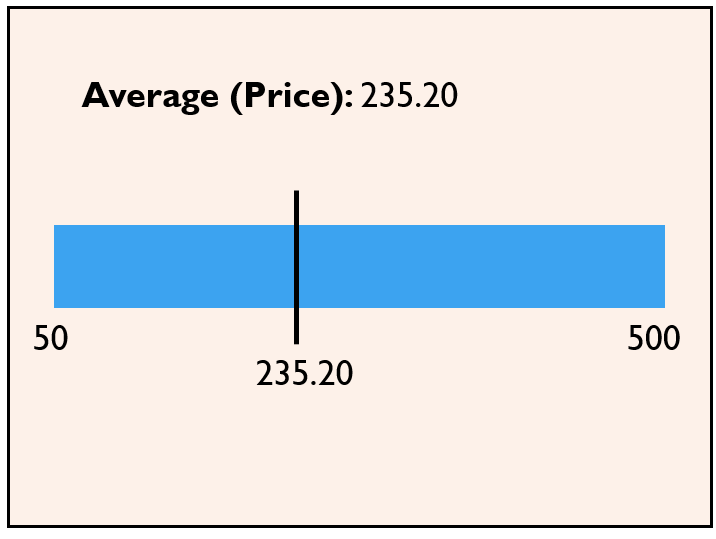
\includegraphics[width=0.20\textwidth]{images/summary.png} &
   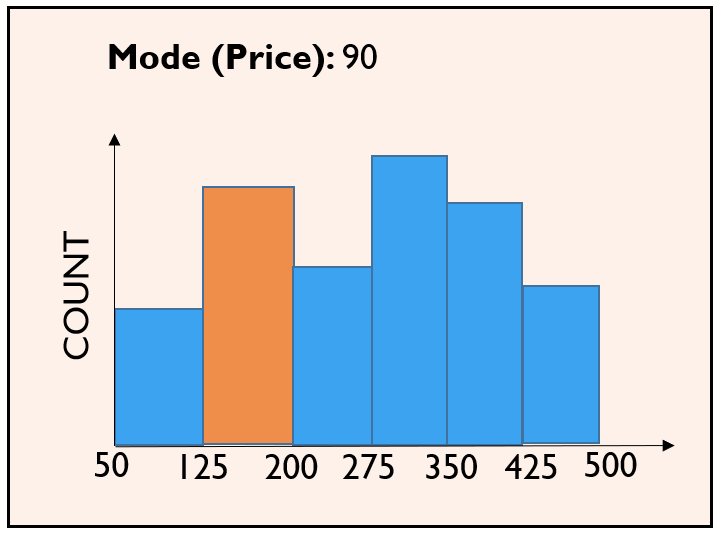
\includegraphics[width=0.20\textwidth]{images/frequency.png} \\
   \textbf{Chart Type:} Summary &  \textbf{Chart Type:} Frequency \\
 \textbf{Representation:} Horizontal bar &  \textbf{Representation:} Histogram \\
 \textbf{Visual Cue:} Vertical line (result) & 
 \textbf{Visual Cue:} Color (highlight) \\ \hline
    & \\
    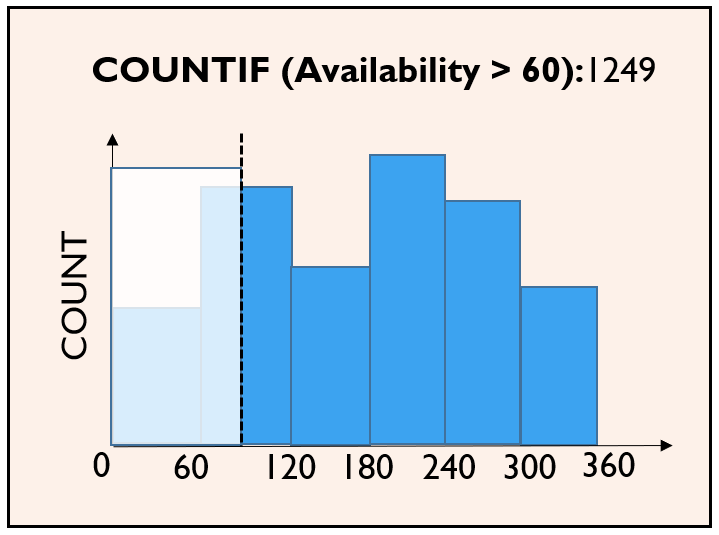
\includegraphics[width=0.20\textwidth]{images/conditional.png}  &
   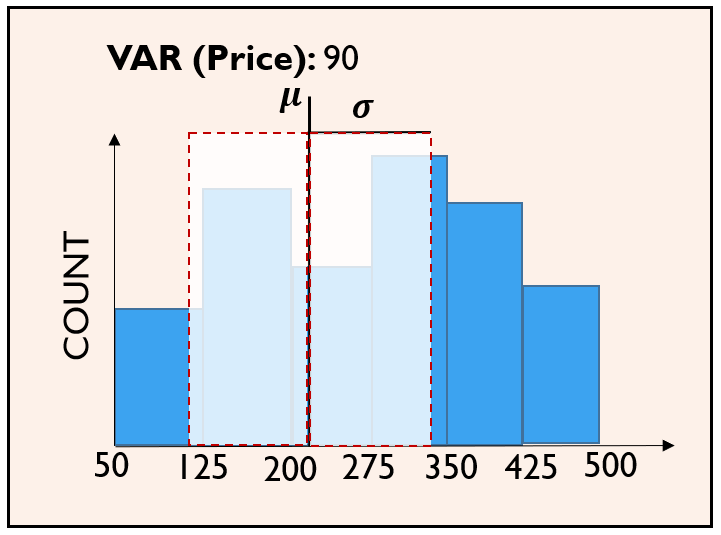
\includegraphics[width=0.20\textwidth]{images/spread.png} \\
      \textbf{Chart Type:} Conditional  &  \textbf{Chart Type:} Spread \\
 \textbf{Representation:} Histogram &  \textbf{Representation:} Histogram \\
 \textbf{Visual Cue:} Vertical line (result), & \textbf{Visual Cue:} Vertical line (mean),\\
Shade (de-emphasize) &  Shade (variance)
\vspace{-5pt}
\end{tabular}
}
\caption{Formula types and their chart representations.}
 \vspace{-15pt}
   \label{fig:agg}

\end{figure}
\subsection{Context Bar}
The context bar consists of two components:
a) a breadcrumb, and b) a navigation history.
The breadcrumb~\cite{breadcrumb} displays the current navigation path (see Figure~\ref{fig:ux}e), thus maintaining the users' navigation context (\textbf{DC6}). Each component of the breadcrumb corresponds to a bin in the user's current navigation path. Therefore, users can visit any bins within the current navigation path by clicking on an appropriate component of the breadcrumb, without having to zoom in or zoom out. \noah also maintains a list of recently visited bins (\textbf{DC6})
(see Figure~\ref{fig:ux}d). \toappendix{If aggregate columns are displayed along with the overview, contents of those columns are updated accordingly (\textbf{DC2}), as users revisit a bin.}

\subsection{Implementation}
We have integrated \noah with {\scshape DataSpread}~\cite{datamodels}, a web-based spreadsheet. The {\scshape DataSpread} back-end maintains the histogram data structure and  supports the aggregate column computation via its built-in formula engine.\toappendix{ To enable seamless integration of the overview with the spreadsheet data, we leverage the hierarchical positional indexes used by {\scshape DataSpread} to access
the spreadsheet data. The index is essentially an order statistics tree~\cite{datamodels} built on the position (\eg row number) of the spreadsheet data. For any given navigation attribute, a new positional index is constructed first. \noah then leverages the positional mapping to access the underlying data corresponding to the navigation attribute and constructs the histogram depicting the overview. Therefore, \noah can be integrated to any spreadsheet and requires only access to the positional mapping structure of that spreadsheet.} The \noah front-end is built with HTML/CSS/JS technologies along with the D3 framework~\cite{d3} for generating charts.







\section{Evaluation Study Design}
\label{sec:study}

In this section, we present the design of a user study
to evaluate whether 
\noah helps address spreadsheet navigational challenges.
\subsection{Study Design and Participants}
\label{sec:study_design}
\new{Our goal is to study the impact of an in-situ navigation plugin for spreadsheets, \noah, on navigation and exploration of data.
Therefore, we decided to compare a \noah-integrated spreadsheet system with a typical, popular one, Excel, across various tasks. Similar domain specific-evaluations have been performed for evaluating various  overview+detail interfaces, \eg database browsing~\cite{north2000snap} or 
tree navigation~\cite{beard1990navigational}. As explained in Section~\ref{sec:related}, the goals and user populations of spreadsheets and TDA tools are quite different. Therefore, we did not consider TDA tools for the comparative study.}
Our study was designed to answer the following questions:
\squishlist
\item {\bf RQ1.} %\sout{How does the addition of an overview help address spreadsheet navigational challenges, with respect to quantitative performance metrics such as speed and accuracy?}
\new{How does integration of an overview plugin like \noah impact a) the completion time and accuracy of various spreadsheet navigational tasks\newsaj{, and b) the usability of spreadsheet systems?}} \saj{SAJ: the survey results are also part of this RQ}
\item {\bf RQ2.} %\sout{How do users make use of the aggregate column results in conjunction with the raw spreadsheet data to analyze data?} 
\new{How do the various components of \noah impact users' navigational experiences?}
%\item {\bf RQ3.} \sout{How does bin customization help users inject domain knowledge in addressing their specific exploration questions compared to the automated overview?} \sout{\saj{How do users utilize additional features of \noah, \eg bin customization, during navigation?}
%\item {\bf RQ4.} \sout{How is the user's subjective satisfaction with \noah compared to traditional spreadsheets?}}  \sout{\saj{How is the user's subjective satisfaction with \noah compared to the traditional spreadsheets when performing navigational tasks?}}
\squishend

\stitle{Study Design.} We conducted a $2 \times 2$ (2 datasets, 2 tools) mixed design within-subject study. The two tools used in the study were: Microsoft Excel, and \noah integrated within {\scshape DataSpread}~\cite{dataspread}. \new{As mentioned previously, we chose Excel for our comparative study because it is the most popular spreadsheet in use today.}
The study consisted of three phases: (a) an introductory phase explaining
the essential features of \noah via a video tutorial, followed by a warm-up session where participants explored a flight dataset~\cite{web:flight} in \noah 
to familiarize themselves with its features,
(b) a quiz phase where the participants first used both the tools
to perform targeted tasks on two different datasets (described later) 
followed by a survey to provide feedback on their impressions about Excel and \noah, and
(c) a semi-structured interview to collect qualitative feedback regarding the quiz phase. 

\stitle{Datasets.} We used two datasets---the birdstrikes (\new{used for evaluating visual data exploration or recommendation tools like Keshif~\cite{yalccin2018keshif} and Voyager~\cite{wongsuphasawat2016voyager}}), and the Airbnb~\cite{web:airbnb} datasets. These datasets were chosen for their understandability to a general audience. The birdstrikes dataset records instances of birds hitting aeroplanes in different US states. The dataset has 10,868 records and 14 attributes (eight categorical, one spatial region, one temporal, four numeric). 
The Airbnb dataset was larger than the birdstrikes dataset. To ensure a fair comparison across tools, we created a sampled version of the original Airbnb dataset with 10,925 records, by uniformly sampling $10\%$ of the records from each US city. This dataset contained 15 attributes (six categorical, two spatial region, one temporal, six numeric).


\stitle{Participants.} We recruited 20 participants (11 female, 9 male) via flyers across the university and via a university email newsletter. 
The average age of the participants was $31.06$ years ($\sigma = 12.44$). 
The participants came from different backgrounds, 
\eg engineering (seven), business (five), administration (five), and natural science (three). 
During recruitment, 
prospective participants filled out an interest form
where they answered questions about their spreadsheet expertise\newsaj{, spreadsheet usage purposes, and spreadsheet operations they typically use}.
Participants were asked to rate their expertise with
different spreadsheet software, \eg Excel and Google Sheets, 
and their frequency of using various spreadsheet 
tasks \eg data management, data analysis, statistical modeling, and what-if analysis.
We also asked participants about their familiarity 
with basic mathematical and statistical spreadsheet functions
as well as advanced operations, \eg pivot table,
 \code{SUBTOTAL}, and conditional formatting. 
\new{To ensure that prior experience with spreadsheets 
didn't affect the performance of participants during the quiz phase}, 
we only recruited participants who rated their experience 
with Excel to be greater than four on a scale of one (no expertise at all) to five (very experienced). 
The selected participants were familiar with performing 
various tasks on spreadsheets, \eg maintaining, tracking, and
analyzing data, making predictions, and performing comparisons. 
All of the participants were familiar with the basic mathematical
and statistical functions supported by Excel. 
Each participant received \$10 per hour at the end of their session.

\subsection{Study Procedure}
\label{sec:procedure}
We now explain each of the phases of our study in more detail.
 
\stitle{Phase 1: Introduction to \noah.}
We began the study by showing a six-minute video tutorial explaining the features of \noah on a dataset of all the flights across the US for January 2018~\cite{web:flight}. The participants then explored the same dataset using \noah to familiarize themselves with the tool for about 10 minutes. The quiz phase began as soon as the participants finished their exploration. \toappendix{Note that we recruited only experienced Excel users for the study and therefore, we did not provide any introduction to Excel.}

\begin{table}[!htb]
\scriptsize
 \vspace{-10pt}
\caption{\newsaj{Quiz tasks for the birdstrikes dataset. The use cases correspond to the task typology discussed in Section~\ref{sec:usage}}}
\label{tab:questions}
\centering
\begin{tabular}{l l l}
\hline
Category & Question & Use case    \\ \hline
steer                & Organize the data by State. How many& \code{locate} $\rightarrow$\\
                     & flights that had damages (damage = 1)& \code{summarize}\\
                     & originated from Florida? \\ 
identify             & How many flights in the currently &\\
                     & visible spreadsheet window  &  \code{identify}\\ 
                     & have damages? & \\
steer                & How many flights that had damages & \code{locate} $\rightarrow$\\
                     & originated from California?                         & \code{summarize}\\ 
\cmpA                & Which state between Florida and &\\
                     & California  has a higher number of & \code{compare}\\ 
                     & flights with damages?    &\\
\cmpB                & Find the state with the most & \code{compare}\\
                     & birdstrike occurrences.  &\\ 
customize            & Organize the data by \emph{altitude}. &\\
                     & What is the average cost of damages & \code{generate}\\
                     &    for altitude bin 0-450?         & \\ \hline
\end{tabular}
\end{table}


\stitle{Phase 2: The Quiz Phase.}
\new{The purpose of the quiz phase was to evaluate the effectiveness of \noah in addressing spreadsheet navigation limitations}. During the quiz phase, 
each participant performed specific tasks on the two datasets in two sessions, using Excel for one and \noah for the other. 
Each session was followed by a survey, described later. We
alternated the order of the datasets between consecutive participants. 
The order of the tools was alternated between every two participants. 
We developed an online JavaScript-based quiz system that recorded user responses and submission times. 
We also recorded the participants’ interactions
with both tools using screen capture software. 
Participants were informed that they can refer to the Internet for help as many times as they wanted. However, due to their familiarity with Excel, none of the participants required external help. 
For reference, we also provided a printed handout to the participants 
that contained screenshots with the features of \noah. 

\emph{Quiz Tasks.} \new{We designed six tasks grouped into four categories: 
steer (two tasks), compare (two tasks), identify (one task), and customize (one task), representing the Table~\ref{tab:scope} use cases \code{locate}, \code{summarize}, \code{compare}, \code{identify}, and \code{generate}, respectively. \newsaj{These use cases are representative of the navigation interactions required for the most frequently issued spreadsheet formulae
~\cite{bradbard2014spreadsheet, lawson2009comparison}.} The tasks were presented in the same order as shown in Table~\ref{tab:questions} for the birdstrikes dataset. The tasks for the Airbnb dataset were similar. The order of the tasks mimics the spreadsheet navigation scenario presented in Section~\ref{sec:usage} \newsaj{where the task complexity increases as the user continues to navigate and analyze the data.}}
%The customize tasks was designed to mimic the scenario where a user would group data subsets of interest and required participants to utilize the bin customization feature. 
%All of these tasks require navigation of the spreadsheet data in the form of either scrolling or steering. 

\newsaj{The steer tasks required the participants to first \code{locate} a data subset and then \code{summarize} the subset by issuing an aggregate operation, \eg \code{COUNTIF}. Following summarization, the identify task required participants to interact with the detailed view and \code{identify} data points within the spreadsheet that satisfy the condition of the first steer task. The purpose of the second steer tasks was to enable the \cmpA task---given the two summaries obtained from the two steer tasks, the \cmpA task asked the participants to \code{compare} the results of both. Then the participants were asked to perform an even more complex comparison, \ie the \cmpB task, which involved comparing the same statistics computed in the two steer tasks of all the data subsets. The purpose of the \cmpB task was to see how increasing the number of subsets would affect navigation. Finally, the customize task was designed to mimic the scenario where the \noah-generated overview doesn't reflect the user preference and a user would group data subsets of interest to create a new overview. (accomplished by utilizing the bin customization feature in \noah).}

%\newsaj{The steer tasks required participants to first \code{locate} a data subset and then issue a formula, \eg \code{COUNTIF}, via steering in Excel to \code{summarize} the subset (accomplished by the aggregate column feature in \noah). Following summarization, the identify task required participants to interact with the detailed view and \code{identify} data points within the spreadsheet that satisfy the condition of the first steer task (accomplished by inspecting the colored spreadsheet cells in \noah). The purpose of the second steer tasks was to enable the subsequent comparison tasks. Given the two summaries obtained from the two steer tasks, the participants were then asked to \code{compare} the results of both, \ie the \cmpA task (accomplished by utilizing the context bar feature of \noah to revisit the results of the first steer task). The \cmpB task involved comparing the same statistics computed in the two steer tasks of all the data subsets. The purpose of the \cmpB task was to see how increasing the number of subsets would affect navigation. Finally, the customize task was designed to mimic the scenario where the \noah-generated overview doesn't reflect the user preference and a user would group data subsets of interest to create a new overview. (accomplished by utilizing the bin customization feature in \noah).}


%As participants use both \noah and Excel to perform these tasks, by examining participants' task performance, we can understand a) how the addition of an overview affect participants' navigation experience (\emph{RQ1}), b) what are the impacts of the individual features of \noah in spreadsheet navigation (\emph{RQ2}), and c) how the participants utilize the features supported by \noah during navigation (\emph{RQ3})

\emph{Survey.} After each session, 
participants rated the corresponding tool used on six metrics: 
confidence, comprehensibility, level of satisfaction, 
ease and speed of use, and ease of learning for spreadsheet navigation, 
on a Likert scale from one (\eg strongly disagree) to seven (\eg strongly agree). 
The survey asked multiple questions related to these metrics, 
15 in total, to ensure reliability. 
Participants were also asked to mention the positive 
and negative aspects of both tools. 
\newsaj{The survey was designed to evaluate \emph{RQ1b}}.

\emph{Evaluation.} 
We evaluated the accuracy and
completion time for each of the six tasks. 
\newsaj{We combined this analysis with qualitative survey, interview, and screen/audio recording data to provide insights that can be corroborated across multiple information sources. Moreover, we analyzed the survey responses to quantify the usability of both Excel and \noah-integrated {\scshape DataSpread}.} 
%For example, we analyzed the video recordings of participants' interaction with the tools during the quiz phase.  

\stitle{Phase 3: Interview Phase.} 
Following the survey, we conducted a semi-structured interview to 
identify participants’ preferred tools for different tasks 
and to understand the reasoning behind their choices. 
We also asked participants to comment on the usefulness of 
different features provided by \noah and Excel. 

\subsection{Study Limitations.}
\newsaj{Our study has several limitations that can be strengthened by future larger-scale and more fine-grained studies. Firstly, our participant pool demographics partially represents the demographics of the general audience intended for \noah. A larger sample with more participants that better represents the spreadsheet user population would have provided more ecological validity to generalize our findings.
}
%While a larger sample with more diverse backgrounds would have allowed us to perform more definitive quantitative analysis, we combined this analysis with qualitative survey, interview, and screen/audio recording data to provide insights that can be explained with multiple information sources.

\newsaj{Next, we only compared the performance of a \noah-integrated spreadsheet with a traditional spreadsheet. We did not evaluate specific spreadsheet features like pivot table and \code{SUBTOTAL} as they violate most of the design considerations proposed in Section~\ref{sec:design}. We discussed their limitations in Section~\ref{sec:related}. Moreover, allowing the participants to utilize the typical spreadsheet operations that they were comfortable with, enabled us to observe how introduction of \noah affected their navigation experience.} 

\new{Finally, we did not isolate the effects of the individual features of \noah to better understand the implications of those. For example, the effect of binned overview (visual clarity versus visual continuity), display layout (screen space trade-off), and
contextual presentation of data (raw text versus chart representation of aggregate columns). However, the goal of the study was to understand participants' navigation experience in the presence and absence of \noah. A more fine-grained study that teases apart the contribution of individual components of \noah is warranted.}


\begin{comment}
\infovis{
\begin{itemize}
    \item Justify the choice of comparing to Excel and note the limitations of that approach (see section 6.1 intro and the {\bf study design paragraph})
    \item Better justify the choice of tasks in the study (see section 6.2 \emph{quiz tasks})
    \item Explain the choice of the four research questions. (see section 6.1 intro)
    \item Provide more details about the study, including reporting intra-participant
    differences (see section 7.2)
\end{itemize}
}
\end{comment}


\section{Results}
\label{sec:results}
In this section, we analyze the quantitative and 
qualitative data collected during the quiz and interview phases 
to address our research questions. 

\subsection{RQ1. Navigation performance of participants}
\label{sec:rq1}
To answer RQ1, we first compare our participants’ task completion times  
and accuracies in \noah and Excel while analyzing the survey response.  
\begin{figure}[t]
   \centering
\begin{tabular}{c c}  %trim=left bottom right top
 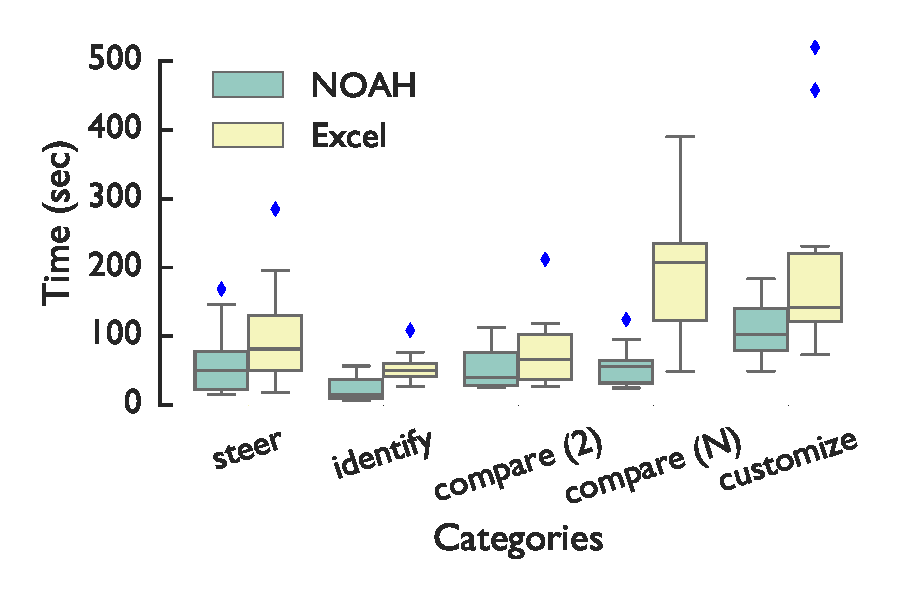
\includegraphics[width=0.23\textwidth,trim={18 37 20 15},clip]{images/bird_box.pdf} &
   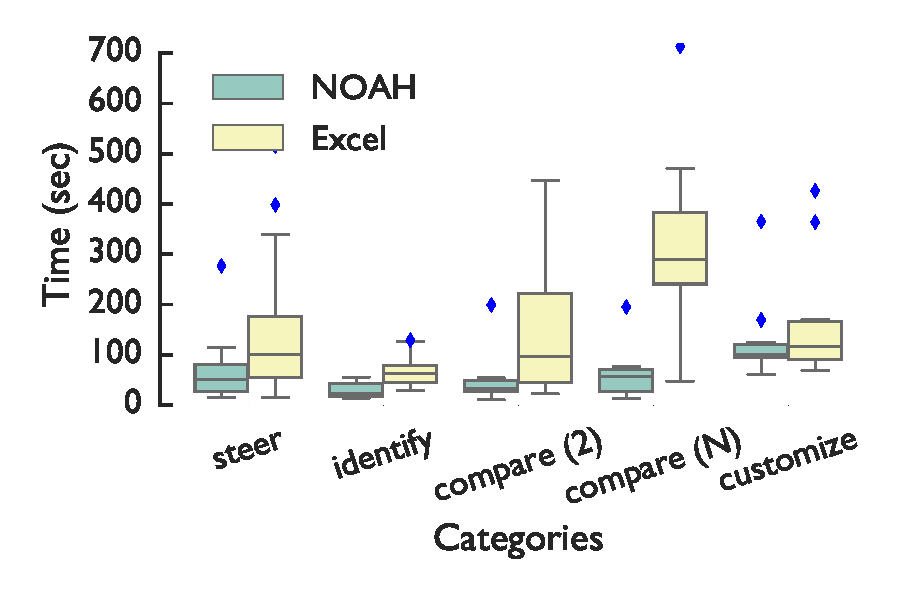
\includegraphics[width=0.23\textwidth,trim={18 37 20 15},clip]{images/airbnb_box.pdf} \\
   \textbf{(a) birdstrikes} & \textbf{(b) airbnb} \\
\end{tabular}
\caption{Submission times per category for each dataset. Median submission times are much smaller for \noah compared to Excel.}
\label{fig:timeBox}
\end{figure}

\subsubsection{Faster navigation without sacrificing accuracy}
In Figure~\ref{fig:timeBox}a and~\ref{fig:timeBox}b, 
we show the distribution of submission times of participants 
for the four task categories, for birdstrikes and Airbnb respectively. 
For most categories, 
\emph{participants' median submission times using \noah 
were less than the fastest submission times using Excel}. This suggests that
the new capabilities offered by \noah
made spreadsheet navigation faster for these tasks. We also analyzed the intra-participant submission time difference, and that supported the aforementioned observations. Overall, majority of the submission times using \noah were faster compared to Excel---19 out of the 20 participants completed at least four tasks in less time using \noah compared to Excel. The submission time differences were more prominent for the steer, identify, and \cmpB tasks. Moreover, for all tasks except customize, the difference in submission times was statistically significant. Both the intra-participant difference and the statistical significance test results are discussed in detail in the Appendix.

\begin{figure}[!htbt]
   \centering
\begin{tabular}{c c} %trim=left bottom right top
   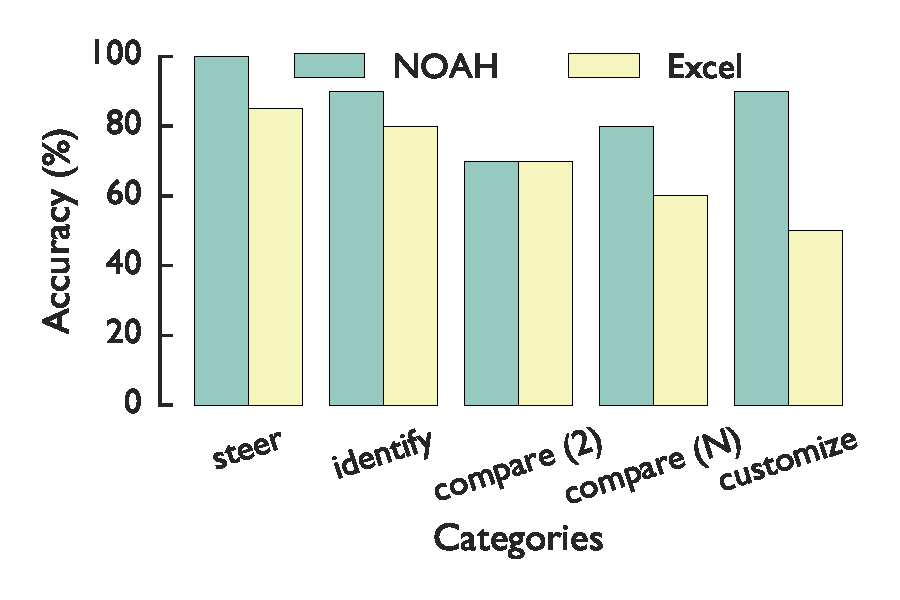
\includegraphics[width=0.23\textwidth,trim={18 35 20 20},clip]{images/bird_accC.pdf} &
   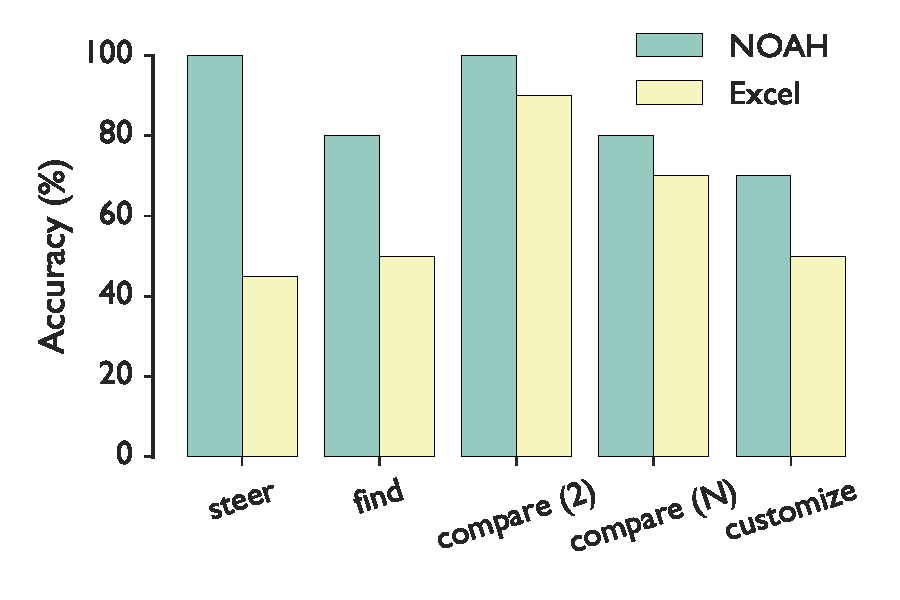
\includegraphics[width=0.23\textwidth,trim={18 35 20 10},clip]{images/airbnb_accC.pdf} \\
   \textbf{(a) birdstrikes} & \textbf{(b) airbnb} \\
\end{tabular}
\caption{Per category accuracy for each dataset. Participants attained higher accuracy while completing tasks in NOAH compared to Excel.}
\label{fig:acc}
\end{figure}
%\subsubsection{Accurate submissions with \noah} 
In Figure~\ref{fig:acc}a and~\ref{fig:acc}b, 
we show the percentage of correct submissions for the four quiz task categories, 
for the birdstrikes and Airbnb datasets, respectively. 
For all the tasks except for the fourth task, \cmpA, for which the accuracy
was the same for both tools, participants 
attained slightly higher accuracy
with \noah compared to Excel. However, the difference in accuracies was statistically significant 
for the steer tasks only (see Appendix). 
\toappendix{Analysis of screen capture for \cmpA 
revealed that between Florida---the correct answer---and California, 
three participants ($P12$, $P13$, and $P20$) out of 20 
chose the latter when using \noah.}

\begin{figure}[!htbt]
    \centering
    %\vspace{-10pt}
    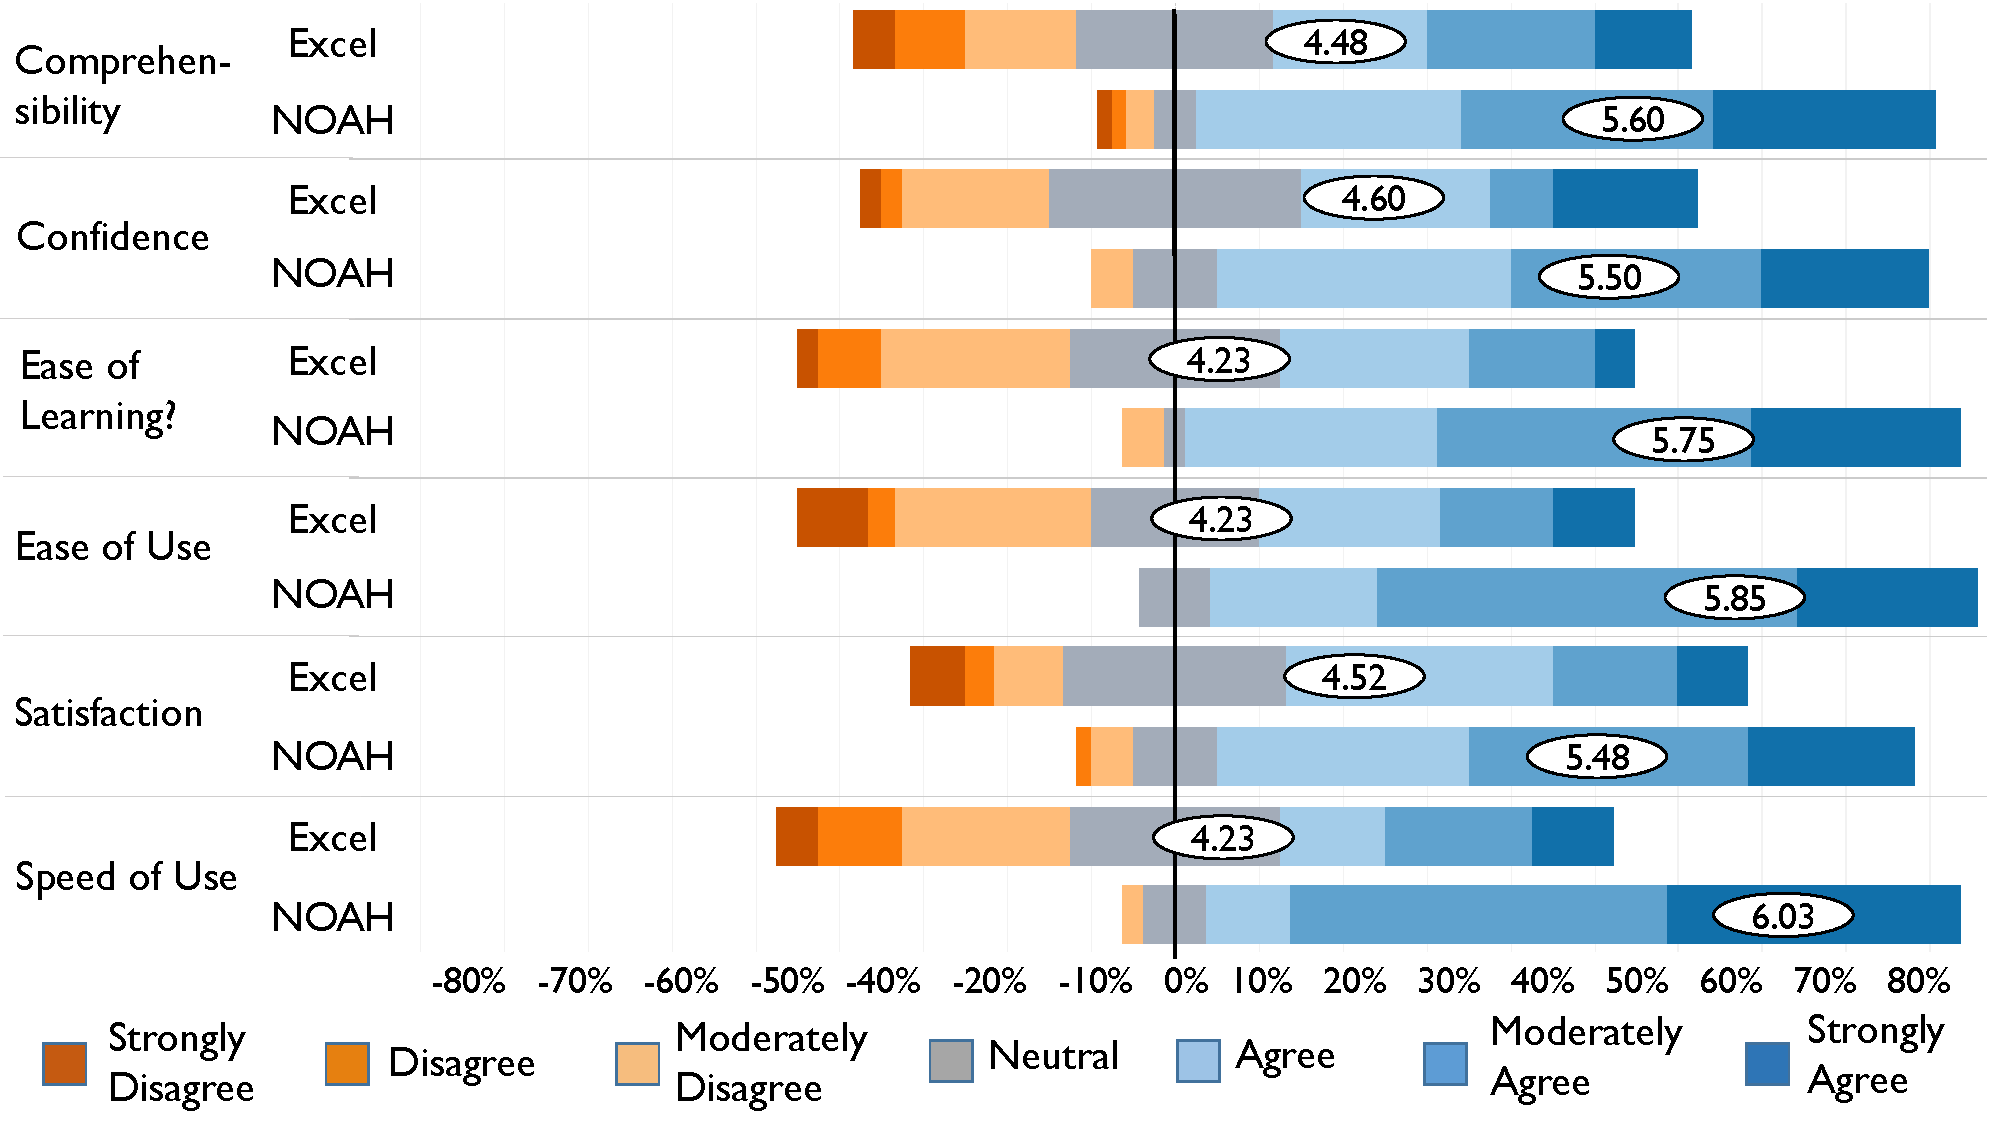
\includegraphics[trim=0 0 0 0,clip,width=\linewidth]{images/survey.pdf}
   \caption{Participants found \noah to be easier to use compared to Excel while being faster in completing tasks involving navigation.}
   \label{fig:survey}
 \end{figure}

\subsubsection{Participants' preferences: \noah VS Excel} 
\saj{Figure~\ref{fig:survey} shows a diverging stacked bar chart representation of the survey results in which participants rated their experience with Excel and \noah. 
For each metric mentioned in Section~\ref{sec:study}, there are two stacked bar charts, one for Excel and one for \noah. Each component within a stacked bar represents the percentage of responses for the corresponding rating, where the ratings are on a scale of one one (strong disagreement) to seven (strong agreement). The average rating for each metric is represented with a white ellipse. Notably, \noah had a higher average rating than Excel for all the metrics. The aforementioned observation was further validated by a statistical significance test---the \emph{Wilcoxon Signed-rank Test} (see Appendix). In particular, participants felt that using \noah was faster and easier 
compared to Excel.}
%Even though the features offered by \noah were new to participants they found it fairly easy to learn. 
\toappendix{We further conducted a statistical significance test---the \emph{Wilcoxon Signed-rank} test---on the survey responses which showed that for all the metrics, the ratings significantly differed by the choice of the tool, \ie \noah or Excel. 
The distribution of the ratings for none of the criteria followed a normal distribution.}

\subsection{RQ2. Impact of \noah and its components on spreadsheet navigation}
\label{sec:rq2}
To answer RQ2, we assessed how \noah components impacted navigation in our study.
%We now discuss how \noah impacted participants' navigation experience compared to Excel.

\subsubsection{Binned Overview}
\stitle{Data navigation at scale.}
\saj{Without an overview, participants found it difficult to 
perform various tasks in Excel. One participant ($P11$) commented---\response{Excel can get overwhelming 
if you have a lot of data in it and sometimes with that data 
finding things can be difficult}. Participants ($N=6$) mentioned 
that they would prefer \noah over Excel when the dataset is large: 
\response{If I just had a large amount of data 
then I would prefer to use \noah because then you 
would be able to see all of it (bins) at once} ($P2$).
\noah's binned overview helped participants comprehend
the overall structure of the data better 
and prioritize the bin they want to visit next, enabling faster navigation. One participant ($P5$) commented: 
\response{I think it was just a little bit easier to navigate 
and find where things were because you could already see what bins had what.} Another participant ($P1$) said:  
\response{I like \noah a lot better. It was a lot easier to look up different data 
and it was a lot quicker too}.}
%Out of 20 participants, 15 preferred \noah for tasks involving navigation. 

\stitle{Enhanced navigation with guided bin customization.} 
\saj{The bin customization feature enabled users to 
personalize the overview based on their specific needs. 
One participant ($P16$) commented: 
\response{I did like the fact that it lets you take a data sheet and, in some way, containerize the stuff you care and the stuff you don't care about.} 
14 out of 20 
participants found the bin customization feature to be useful. 
Participants preferred the feature to Excel's filtering feature 
when working with numeric data---\response{That was so much easier in \noah 
than it was in Excel to be able to specify the range that you wanted it to go in} ($P17$). Our analysis of the video recordings revealed that, for the birdstrikes dataset in Excel, the customize task involved filtering out the desired values from a total of 451 unique values. As a result, participants had to manually filter a large number of values and took more time
to submit their responses compared to \noah when they were able to use the bin customization feature. However, the time taken for this task was higher than  other tasks in \noah, as
it required participants to restructure the overview
before any calculation could be performed.
Unfamiliarity with customization
operations also contributed to higher task completion times.}

\stitle{Unfamiliar interactions.} \saj{Participants were unfamiliar with the bin customization feature.
This unfamiliarity led to some participants ($N=5$ out of 20) 
preferring Excel over \noah. One participant ($P11$) commented: \emph{Since I'm not used to spreadsheet data being presented that way, it took a little bit of getting used to.} Participants found some of the terminology 
used in the interface---\eg explore, bin---quite 
unfamiliar ($N=14$). 
Moreover, two participants didn’t understand how the bins were constructed.}

\stitle{Overview presentation across data types.}
\saj{Although participants appreciated the binned representation of the overview for numeric data, a number of participants ($N=6$) stated that they would've preferred a pivot table-like single level overview for categorical data where each bin corresponds to one item. One participant ($P13$) commented: \response{I would prefer it start with all the bins split, and then I can merge them as I want.} Another participant ($P4$) said---\response{When I started, it (\noah) had already grouped them, I think, alphabetically. So, that creates an extra step in that I then have to go split them and then re-merge them.}} 

\subsubsection{Aggregate Column}
\stitle{Ease of issuing formulae.} 
\saj{The steer tasks required participants 
to issue a \code{COUNTIF} formula on a data subset. 
Participants found scrolling and steering in Excel 
to be cumbersome while issuing formulae---\response{The one thing
with Excel is I always try to go to the bottom of the data 
and type in the formula, and with something really long like this, 
the scrolling is a little bit cumbersome} ($P4$). 
With \noah, participants avoided
(a) scrolling by using clicking or zooming operations, 
and (b) steering by performing aggregate operations on the overview. Participants ($N=13$) found it easier to issue formulae using the aggregate column feature.
One participant ($P3$) commented: 
\response{And that creates convenience sort of because then you don't have to memorize anything and using the system becomes easier.} 
Another participant ($P13$) commented: \response{There were some formulas to calculate, that were definitely easier in \noah because the aggregate column did all the work and showed me the results.} However, two participants found the aggregation operations 
applied on the bins to be opaque compared to Excel 
where a user can directly manipulate the formula. 
}

\stitle{Higher efficiency in issuing formulae.} 
\saj{While the accuracies and submission times for the steer tasks in Excel varied significantly across datasets, using \noah, participants exhibited higher accuracies and faster submission times irrespective of the dataset (see Figure~\ref{fig:timeBox} and~\ref{fig:acc}). The automated and steering-free aggregate column feature of \noah contributed to high accuracies (100$\%$) for the steer tasks.  One participant ($P12$) commented: \response{With \noah, 
you don't have to highlight every number versus Excel where you actually have to select everything.} All of the 14
inaccurate submissions with Excel involved steering incorrect spreadsheets regions. 11 of the inaccurate submissions were with the Airbnb dataset. However, in \noah, participants were able to avoid steering by utilizing the aggregate column feature. Analysis of screen recordings of Excel usage
revealed that for birdstrikes dataset, several participants 
used the \emph{autosum}
feature to quickly count the number of $1$'s in a binary-valued column that was involved in the steering task. Summing up
binary values is equal to the number of $1$'s in the collection. 
Other participants used the status bar at the
bottom of the spreadsheet that displayed the sum 
of the cells in the selected column. 
In both cases, participants avoided steering the data. 
On the other hand, for Airbnb dataset, participants 
could not use these shortcuts as the column that was involved in the steering task was non-binary 
(it had 365 different values). Participants, at times, steered incorrect regions, resulting in inaccurate responses for the task.  
Therefore, the participants’ ability to avoid steering 
depended on the data type. 
Failure to avoid steering often led participants
to selecting an incorrect range of data ($N=14$), resulting in incorrect
responses.}

\subsubsection{Detailed View}
\stitle{Accelerated data inspection.} 
\saj{For the \emph{identify} task, 
participants had to skim through all the cells 
in the current window in Excel, 
resulting in higher completion times. 
%Again, participants had to skim over binary values when counting in birdstrikes versus non-binary values for Airbnb, resulting in even higher completion times for the latter. 
Even though Excel provides a conditional formatting feature, that adds one additional step when performing the \emph{idenitfy} task. 
In \noah, participants benefited from having visual cues in the form of colored cells, helping them relate the aggregate column with the raw data---\emph{You didn't have to do any additional steps and it was a visual cue right there, made it very quick to count it up ($P17$).} Another participant ($P9$) commented---\response{In Excel, you would have to do your own condition of formatting. But you have to build that every time  you need to ask a question. This one (\noah) at least something is pre-built in, and you can easily count.} However, one participant ($P3$) pointed out the fact that, when the data corresponding to the bin does not fit in the screen, they had to scroll through the data to identify relevant information.}
%Out of 20 participants, 16 participants preferred the automatic data highlighting feature of \noah while performing the \emph{identify} task. Moreover, the colored cells focused their attention to relevant regions within the spreadsheet Another participant ($P5$) mentioned the fact that some of the color choices would make \noah unusable for the colorblind population.}



\subsubsection{Context Bar}
\stitle{Utilizing history to avoid repeated execution.}
\saj{For the \cmpA task, participants utilized the context bar to navigate to the previously visited bin for the first steer task. As \noah automatically materialized the aggregate summaries of a previously visited bin, participants were able to view the aggregate column values instantly without having to repeat the same command. However, as Excel did not preserve any navigation history, participants had to re-execute the first steering operation. As a result, the submission times for \cmpA tasks were lower in \noah compared to Excel (see Figure~\ref{fig:timeBox}). One participant ($P16$) commented---\response{Once I got familiar with the interface, it was easy to just say, I want to see this state, and I like that fact that like automatically it goes into the bins on NOAH, gave me summary information.} Another participant ($P9$) said---\response{Noah was easy to find and compare and toggle in between.} }

\stitle{Visual discontinuity during navigation.} 
\saj{For \cmpB tasks, participants 
had to perform $N$ comparisons in \noah while issuing the aggregate column operation once. However, comparison among $N$ bins resulted in increased visual discontinuity. This lead to some ($N=4$ out of 20) incorrect submissions. In excel, the experience was worse, as the participants had to perform $N$ steering tasks. As a result, in Excel, \cmpB task submission times were very high compared to \cmpA tasks (see  Figure~\ref{fig:timeBox}). In addition, the accuracies of the \cmpB task in Excel were extremely low.}

%The completion times were faster in \noahthan in Excel, irrespective of the comparison tasks and datasets. \emph{\noah offers three additionalbenefits apart from avoidance of steering that may have contributed to such improvement}:
%a) participants used the navigation features to access and compare different subsets of data quickly, 
% b) participants did not need to reissue the aggregation formula for any of the bins they navigated to, and 
%c) participants used the value bars presented along with the results in the aggregate column to visually compare different subsets.
%For \cmpB tasks, the number of subsets to be compared was  higher in birdstikes (50) compared to Airbnb (16). As a result, participants exhibited lower accuracy for birdstrikes when using Excel. In \noah, all the participants first split all the bins to create $N$ bins each corresponding to one state. Then participants panned across the overview to find the desired bin as they compared the values. Even in \noah, comparisons between multiple values resulted in increased visual discontinuity leading to some ($N=4$ out of 20) incorrect submissions.


%!TEX root = main.tex
\section{Discussion and Conclusion}
\label{sec:discuss}
\new{\noah represents our 
first step towards a general purpose spreadsheet navigation plug-in to make spreadsheets more effective
when exploring datasets that are increasingly the norm. 
Using \noah, users can get a bird's eye view of the data, with the ability to scroll or seek
additional details on demand via a multi-granularity overview, as well as employ
aggregation
in-situ, which eliminates cumbersome steering operations. Quantitatively, we find that \noah speeds up navigation without compromising accuracy. Qualitatively, study participants identify it as positively impacting their experience while overviewing and navigating large datasets, and issuing formulae. However, the user study revealed some limitations of \noah. Moreover, the study design itself had some limitations. In this section, we discuss these limitations and propose extensions to address these limitations as well as enhance the capabilities of \noah.}

\subsection{User Study Limitations}
Our study has a few limitations that can be strengthened by future larger-scale and finer-grained studies. 

\stitle{\new{Insufficient coverage of participant demographics.}} \new{Our participant pool demographics only partially represents the demographics of the general audience intended for \noah. A larger sample with more  participants with a range of skill-sets and backgrounds that better represents the spreadsheet user population would have provided more ecological validity to generalize our findings.}
%While a larger sample with more diverse backgrounds would have allowed us to perform more definitive quantitative analysis, we combined this analysis with qualitative survey, interview, and screen/audio recording data to provide insights that can be explained with multiple information sources.

\stitle{\new{Lack of targeted comparisons with advanced spreadsheet features.}} \new{We only compared the performance of a \noah-integrated spreadsheet with a traditional spreadsheet. We did not evaluate specific spreadsheet features like pivot table and \code{SUBTOTAL} as they violate most of the design considerations proposed in Section~\ref{sec:design}; we discussed their limitations in Section~\ref{sec:related}. We instead allowed the participants to freely use any spreadsheet operations that they were comfortable with (including the advanced ones), enabling us to observe how introducing a plug-in like \noah affected their navigation experience. However, a future study targeted at evaluating the pros and cons of these features for spreadsheet navigation would be valuable.} 

\stitle{\new{Isolated evaluation of \noah components.}} \new{While we did present the impact of various components of \noah in Section~\ref{sec:rq2}, we did not isolate the effects of individual features during our study. For example, we did not study the effects of the binned overview (visual clarity versus visual continuity), display layout (screen space trade-off), and
contextual presentation of data (raw text versus chart representation of aggregate columns) in isolation. A more fine-grained study that teases apart the contribution of individual components of \noah is warranted.}

\subsection{Limitations of \noah and Possible Enhancements}
While we alluded to some limitations of \noah in Section~\ref{sec:results}, we now discuss these in more detail and how we can possibly overcome them.

\stitle{\new{Lack of transparency and documentation of new interactions.}} \new{Several operations in \noah 
are quite different from typical spreadsheet interactions, \eg zooming or bin customization. Moreover, participants found some of the terminologies, \eg explore or bin, to be rather different from typical spreadsheet terminologies, which took some getting used to (see Section~\ref{sec:rq2}). In addition, some participants complained about the lack of explanation surrounding the overview construction and aggregate column computation. In the future, these issues can be addressed by using more relatable terminologies and improved documentation.}

\stitle{\new{Deviation from the spreadsheet look and feel.}}
\new{A couple of participants ($P2$ and $P11$) mentioned that the aggregate column results hides the actual spreadsheet formula and they would prefer some visual cues that highlight the corresponding formula underlying each bin. Subsequent versions of \noah can  
display the appropriate formula for each bin as users hover
over the corresponding cell on the aggregate column\cut{making the output more relatable to typical spreadsheet formula results}. The aggregate column feature can be further enhanced by enabling users to issue user defined formulae, a feature requested by a number of participants ($N=5$). Another feature that can be made more similar to spreadsheet interaction semantics is the bin customization operation. Currently, this operation in \noah is performed from a menu bar, adding an additional step. The bin splitting and merging operations can be made more similar to how spreadsheet cells are split or merged---in Excel, these operations are direct and only require a single click. Similar direct adjustment of data grouping strategies have been explored for visualization tools~\cite{sarvghad2018embedded} and can be adapted to this setting.} 

\stitle{\new{Absence of bespoke overview representations for various data types.}} \new{The experience 
surrounding the construction
of the overview
can be further improved, especially for categorical data.
Currently, the bins of the overview
can be customized
only after the overview is constructed.
Providing the users
the ability to
select the representation
(similar to bin customization)
of the overview at the outset could have possibly addressed this issue.
Understanding the impact of these
representation choices for the overview
is an interesting open question.}

\subsection{Additional enhancements}
\label{sec:discuss_additionational}
We now discuss other functionalities that can be introduced to further enhance the capabilities of \noah.

\stitle{\new{Broadening the scope of overview-spreadsheet coordination.}} 
\new{Spreadsheet users often perform various edit operations, 
\eg updating values, adding/deleting rows/columns. 
However, our current \noah implementation assumes the data to be read-only. 
In our next version, we can add support for
propagating spreadsheet updates to the overview. 
Moreover, the charts displayed in an \emph{aggregate column} are non-interactive, 
\ie users cannot interact with the charts to visually look up relevant or 
interesting data points within the spreadsheet. 
In the future, we plan to extend \noah to support visual querying 
through the charts in an aggregate column, similar to multi-modal linked selections in Keshif~\cite{yalccin2018keshif}.}

\stitle{\new{Enabling more flexible overview binning.}} \noah currently constructs the overview on a single attribute. We can add support for multi-attribute navigation (\eg explore the Airbnb data by city and neighborhood), and multi-level navigation (\eg explore the neighborhoods after zooming into a specific city in the Airbnb data). Furthermore, bin customization currently supports changing the bin boundaries only, while maintaining the current order. Supporting user-defined ordering to allow arbitrary reshuffling of the bins can be another enhancement.\toappendix{ However, such modification will require a redesign of the histogram based data structure since the ordering property will not hold anymore.Finally, a complete characterization of the spreadsheet operations that can be supported by \noah is another open question, for example, other operations that involve working with subsets of spreadsheet data, \eg sorting, filtering, copy-pasting, can also be supported by \noah.} 

\stitle{\new{Supporting other spreadsheet operations.}} \new{Spreadsheet operations that involve working with subsets of the data, \eg sorting, filtering, copy-pasting, can be supported by \noah, but our current implementation does not support them. Future versions would support such operations as well. Other enhancements include adding annotations, \eg visual cues, text, to the overview and then exporting the customized overview for presentation or reporting---a required feature for information seeking tools~\cite{shneiderman2003eyes}.}

\stitle{\new{Supporting navigation for semi-structured data.}} \noah operates only on tabular data.
However, spreadsheets can be semi-structured---formulae 
and text can be interspersed with tabular data. 
\new{In such cases, NOAH can be used to support exploration and zooming for each such tabular region independently, supported by an overall overview (akin to a map-based panning tool) for users to select which tabular region they want to explore in detail.}
We can leverage existing work on spreadsheet table detection~\cite{tablesense}, 
and property identification~\cite{chen2017spreadsheet} 
to \new{support such extensions}.  

\stitle{\new{Achieving interactive scalability beyond traditional spreadsheet limits.}} 
The current version of \noah addresses the perceptual 
scalability challenges while navigating 
Excel-scale (one million rows) data. 
As modern spreadsheets continue to support 
increasingly larger datasets---{\scshape DataSpread}~\cite{datamodels} 
supports one billion rows---the interactions proposed in this paper may violate the interactive response time bound of 500 ms~\cite{liu2014effects}. This opens the door to a new set of research challenges that may range from approximate query processing to progressive data analytics.




% if have a single appendix:
%\appendix[Proof of the Zonklar Equations]
% or

% use appendices with more than one appendix
% then use \section to start each appendix
% you must declare a \section before using any
% \subsection or using \label (\appendices by itself
% starts a section numbered zero.)
%


%\appendices
%\section{Proof of the First Zonklar Equation}
%Appendix one text goes here.

% you can choose not to have a title for an appendix
% if you want by leaving the argument blank
%\section{}
%Appendix two text goes here.


% use section* for acknowledgment
\ifCLASSOPTIONcompsoc
  % The Computer Society usually uses the plural form
  %\section*{Acknowledgments}
\else
  % regular IEEE prefers the singular form
  %\section*{Acknowledgment}
\fi


%The authors would like to thank...


% Can use something like this to put references on a page
% by themselves when using endfloat and the captionsoff option.
\ifCLASSOPTIONcaptionsoff
  \newpage
\fi



% trigger a \newpage just before the given reference
% number - used to balance the columns on the last page
% adjust value as needed - may need to be readjusted if
% the document is modified later
%\IEEEtriggeratref{8}
% The "triggered" command can be changed if desired:
%\IEEEtriggercmd{\enlargethispage{-5in}}

% references section

% can use a bibliography generated by BibTeX as a .bbl file
% BibTeX documentation can be easily obtained at:
% http://mirror.ctan.org/biblio/bibtex/contrib/doc/
% The IEEEtran BibTeX style support page is at:
% http://www.michaelshell.org/tex/ieeetran/bibtex/
\bibliographystyle{IEEEtran}
% argument is your BibTeX string definitions and bibliography database(s)
\bibliography{ref}
%\bibliography{IEEEabrv,../bib/paper}
%
% <OR> manually copy in the resultant .bbl file
% set second argument of \begin to the number of references
% (used to reserve space for the reference number labels box)
%\begin{thebibliography}{1}
%\end{thebibliography}

% biography section
% 
% If you have an EPS/PDF photo (graphicx package needed) extra braces are
% needed around the contents of the optional argument to biography to prevent
% the LaTeX parser from getting confused when it sees the complicated
% \includegraphics command within an optional argument. (You could create
% your own custom macro containing the \includegraphics command to make things
% simpler here.)
%\begin{IEEEbiography}[{\includegraphics[width=1in,height=1.25in,clip,keepaspectratio]{mshell}}]{Michael Shell}
% or if you just want to reserve a space for a photo:

\begin{IEEEbiography}{Michael Shell}
Biography text here.
\end{IEEEbiography}

% if you will not have a photo at all:
\begin{IEEEbiographynophoto}{John Doe}
Biography text here.
\end{IEEEbiographynophoto}

% insert where needed to balance the two columns on the last page with
% biographies
%\newpage

\begin{IEEEbiographynophoto}{Jane Doe}
Biography text here.
\end{IEEEbiographynophoto}

% You can push biographies down or up by placing
% a \vfill before or after them. The appropriate
% use of \vfill depends on what kind of text is
% on the last page and whether or not the columns
% are being equalized.

%\vfill

% Can be used to pull up biographies so that the bottom of the last one
% is flush with the other column.
%\enlargethispage{-5in}

\appendix  % for no appendix heading
% do not use \section anymore after \appendix, only \section*
% is possibly needed
In this supplementary material we highlight the use cases that \noah
is suited for, the in-situ chart representations within
the overview, \noah’s underlying system architecture,
and statistical significance results from our user study.
\section*{\noah Use Cases}
As mentioned in Section~\ref{sec:design}, the goal of designing 
an overview interface is to 
not only enable seamless navigation 
but also to facilitate functionalities to help users visually seek information about the data. Therefore, we draw parallels to the typology of abstract visualization tasks~\cite{brehmer2013multi} to identify the use cases that \noah is best suited for. 
We are specifically interested in exploring the different task purposes mentioned in the typology. The task purposes can be specified at three different levels: consume and produce (high-level), search (mid-level), and query (low-level). Table~\ref{tab:scope} captures all three levels and highlights where \noah can be used.

At a very high level, users may utilize \noah to verify some phenomenon in the data (\code{discover}) or consume the data for casual interest (\code{enjoy}). Example of \code{discover} includes a journalist trying to verify whether listings in Airbnb are run as hotels (see Section~\ref{sec:usage}). 
Moreover, users may utilize the overview to communicate details about the data (\code{present}). 
However, visualization tools are more suitable for such a purpose. 
Finally, users can customize (\code{create}) the overview to fit their exploration purpose. Here, the high-level goal is to \emph{Produce} a new representation. 
However, the present version of \noah does not allow users to add annotations, \eg visual cues, texts, to the overview (\code{annotate}).

Regardless of the high-level purposes, users may want to find elements of interest in the overview (\emph{search}) and seek additional details about those elements (\emph{query}). 
In Section~\ref{sec:ui}, we discussed the features and interactions supported by \noah and showed how these interactions enable users to \emph{search} and \emph{query} the data. Users can \code{browse} and \code{explore} the data using navigational operations, \eg clicking and zooming, to find elements of interest. 
Note that if users know either the identity or location of the information they are searching (\eg the name of the city in the Airbnb data), 
they can simply use traditional spreadsheet operations like \emph{VLOOKUP} (\code{lookup}) or \emph{CTRL+F} (\code{locate}) (see Table~\ref{tab:scope}). 
On the other hand, clicking or zooming is suitable when the identity or location of the information is unknown. Therefore, NOAH complements spreadsheets in accomplishing users’ \emph{search} goal via navigational operations. 
Once the user finds the elements of interest, they can further \code{summarize} the elements via aggregate columns, \code{compare} those elements, and \code{identify} the raw data corresponding to the summaries in the spreadsheet.

\section*{Explaining the Chart Representations}

In this section, we explain the chart representation of all the
formula categories discussed in Section~\ref{sec:ui},
also displayed in Figure~\ref{fig:agg}.

\stitle{Summary.} The result of a \emph{summary} formula,
\eg \code{AVERAGE}, is depicted using a horizontal bar.
The bar represents
the range of the data subset the bin spans
with the minimum and maximum values
annotated within the chart. A vertical line is used to highlight
where the result lies within the range.
   
\stitle{Conditional.} The result of a \emph{conditional} formulae,
\eg \code{COUNTIF}, is depicted using a histogram.
The histogram captures the distribution of the attribute,
on which the formula has been applied,
\eg the \emph{availability} attribute discussed
in Section~\ref{sec:usage}.
Shading is used to de-emphasize data ranges
that do not satisfy the condition. A vertical line is used to highlight
where the result lies within the distribution.

\stitle{Frequency.} The result of a \emph{frequency} formula,
\eg \code{mode}, is also depicted using a histogram.
The bin in the histogram
that contains the result is rendered with ``orange'' color.
A vertical line is used to highlight
where the result lies within the distribution.

\stitle{Spread.} Finally, the result of a \emph{spread} formula,
\eg \code{mode}, is depicted using a histogram.
A similar shading technique as the \emph{conditional} formula is used to highlight the standard deviation. The mean of the is highlighted using a vertical line.

In the chart representation mode,
each entry of the aggregate column
contains one additional visual cue---a color bar
with shades of green on
the right of the chart (see Figure~\ref{fig:customize}).
The darker the color, the higher the value corresponding to that entry. 
Users can utilize the color intensity
to compare the results among different aggregate column entries.

\section*{Implementation and  Architecture}
\label{sec:sys}
In this section, we provide an overview of the infrastructure of \noah. 
We integrate \noah as a data exploration plugin within{\scshape DataSpread}~\cite{dataspread}, 
an open-source scalable web-based spreadsheet.

\subsection{Underlying Data Structures}
As explained in Section~\ref{sec:ui}, the underlying data structure representing the overview is an in-memory equi-depth histogram. 
\noah constructs the histogram on demand based on the navigation attribute. 
In the beginning, only the highest granularity bins are constructed. 
As users perform ad-hoc interactions on the data, the interface is updated on the fly. 
For example, when a user zooms into a specific bin, 
\noah again constructs an equi-depth histogram 
on the data corresponding to that bin on demand.
To enable seamless integration of the overview 
with the spreadsheet data, we leverage the hierarchical positional indexes
used by {\scshape DataSpread}~\cite{datamodels} to access
the spreadsheet data. 
The index is essentially an
order statistics tree~\cite{datamodels} 
built on the position (\eg row number) of the spreadsheet data. 
For any given navigation attribute, a new positional index is constructed first. 
\noah then leverages the positional mapping to access the underlying data corresponding to the navigation attribute and constructs the histogram depicting the overview. 
Each bin in the histogram maintains positional information regarding its elements, \ie starting and ending index of each unique element in the bin (\eg cities in the Airbnb data).  
Therefore, \noah can be integrated into any 
spreadsheet and requires only access to the positional mapping structure of that spreadsheet.

\subsection*{System Architecture}

\begin{figure}
    \centering
    %\vspace{-10pt}
    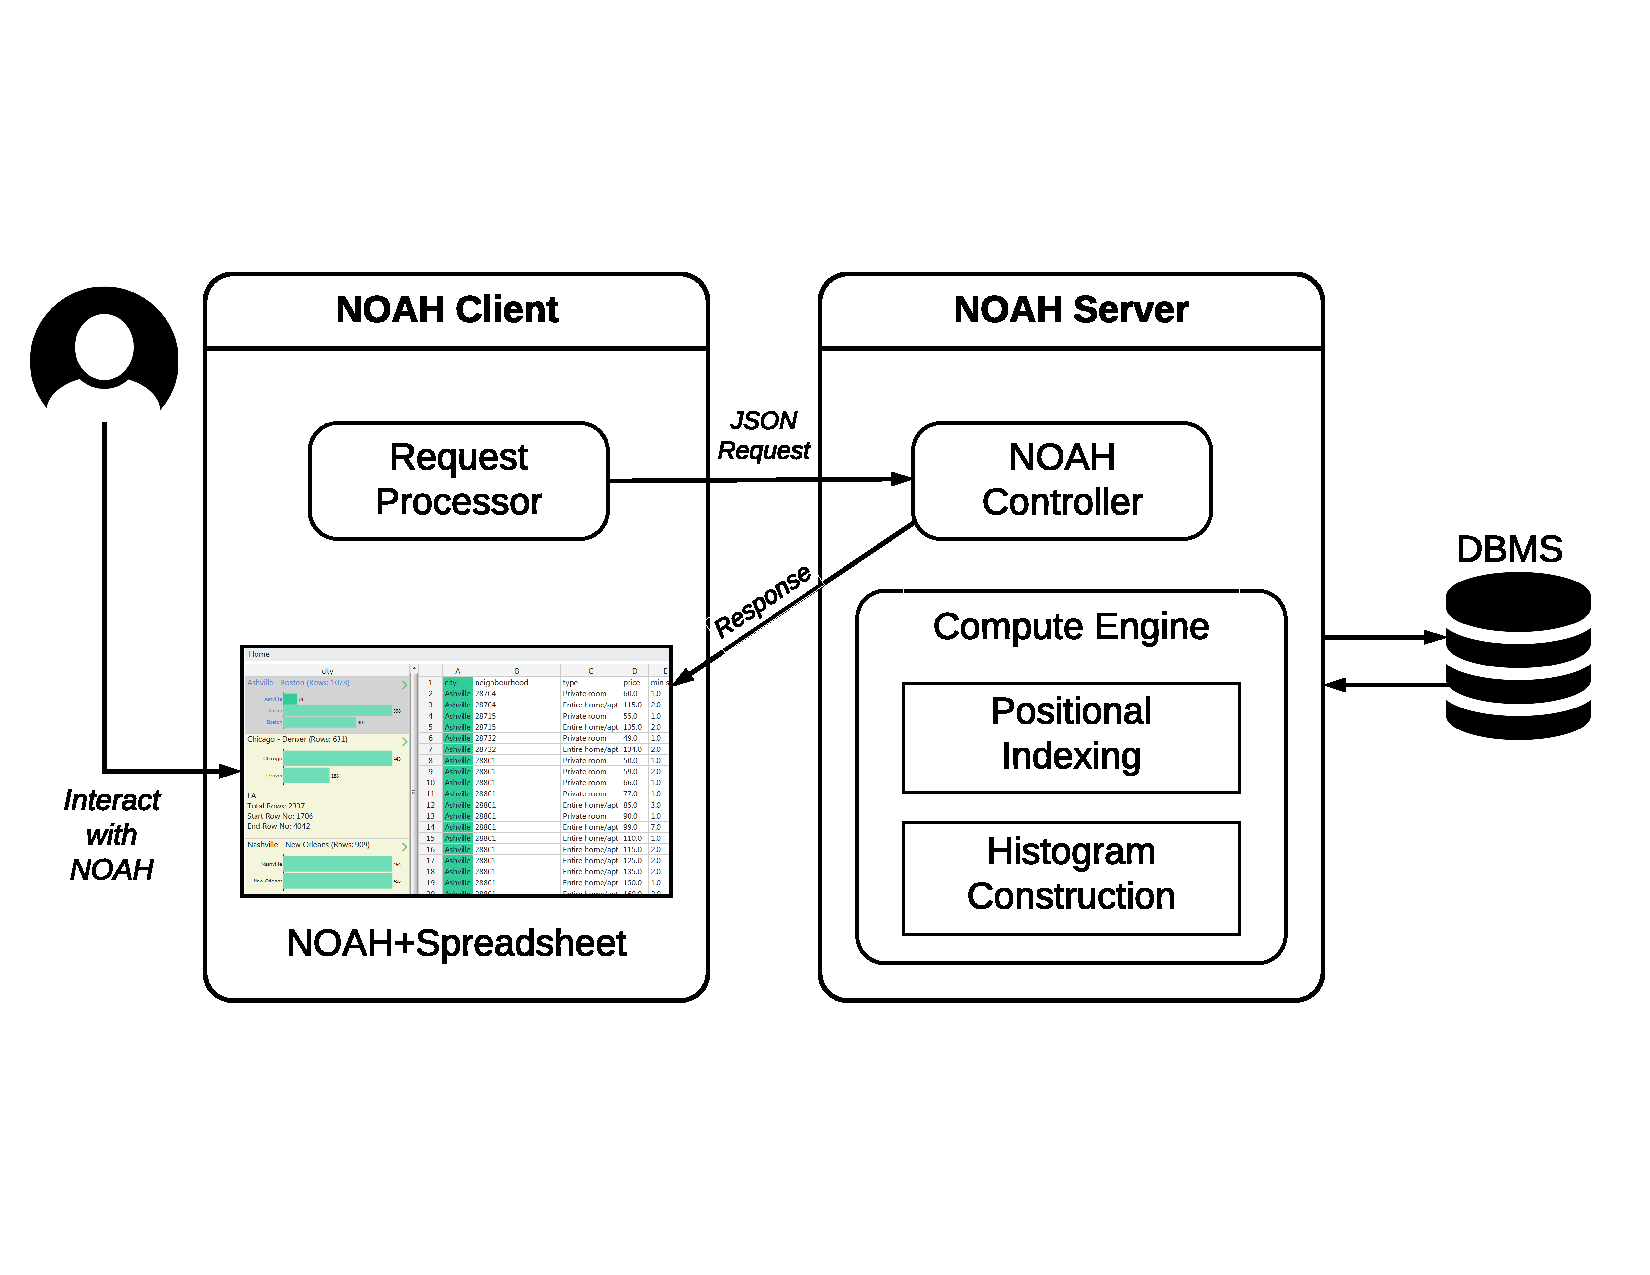
\includegraphics[trim=0 4cm 0 3cm,clip,width=\linewidth]{images/arch.pdf}
   \caption{System architecture.}
   \label{fig:arch}
 \end{figure} 

We now explain the system architecture of \noah. 
The \noah client is a web-based front-end that captures user input and renders both the navigation interface and the spreadsheet 
based on the results returned by the back-end. 
The front-end is responsible for capturing user input and rendering components of the navigation interface, \ie overview, aggregate column, and context bar. 
Given any interaction by the user on the front end, 
the \emph{request processor} issues a request to back end.
The back end navigation controller receives the request from the front end. 
After processing the request that corresponds to some front-end user interaction, 
the \emph{request processor} sends a response to the front-end encoded in \emph{json}. 
For requests involving the spreadsheet, \eg scrolling, 
the \emph{request processor} leverages the \emph{positional index} 
to access the spreadsheet data. 
For requests involving the navigation interface, \eg zoom in/out, 
the \emph{request processor} leverages the \emph{compute engine} to manage the equi-depth histogram on demand. 
The compute engine is also responsible for processing analytical operations. We leverage {\scshape DataSpread}’s built-in formula engine to support the analytical operations.


\section*{Results}
In this section, we evaluate the statistical significance of the task performance results and survey responses presented in Section~\ref{sec:results}. 
\begin{figure}
    \centering
    %\vspace{-10pt}
    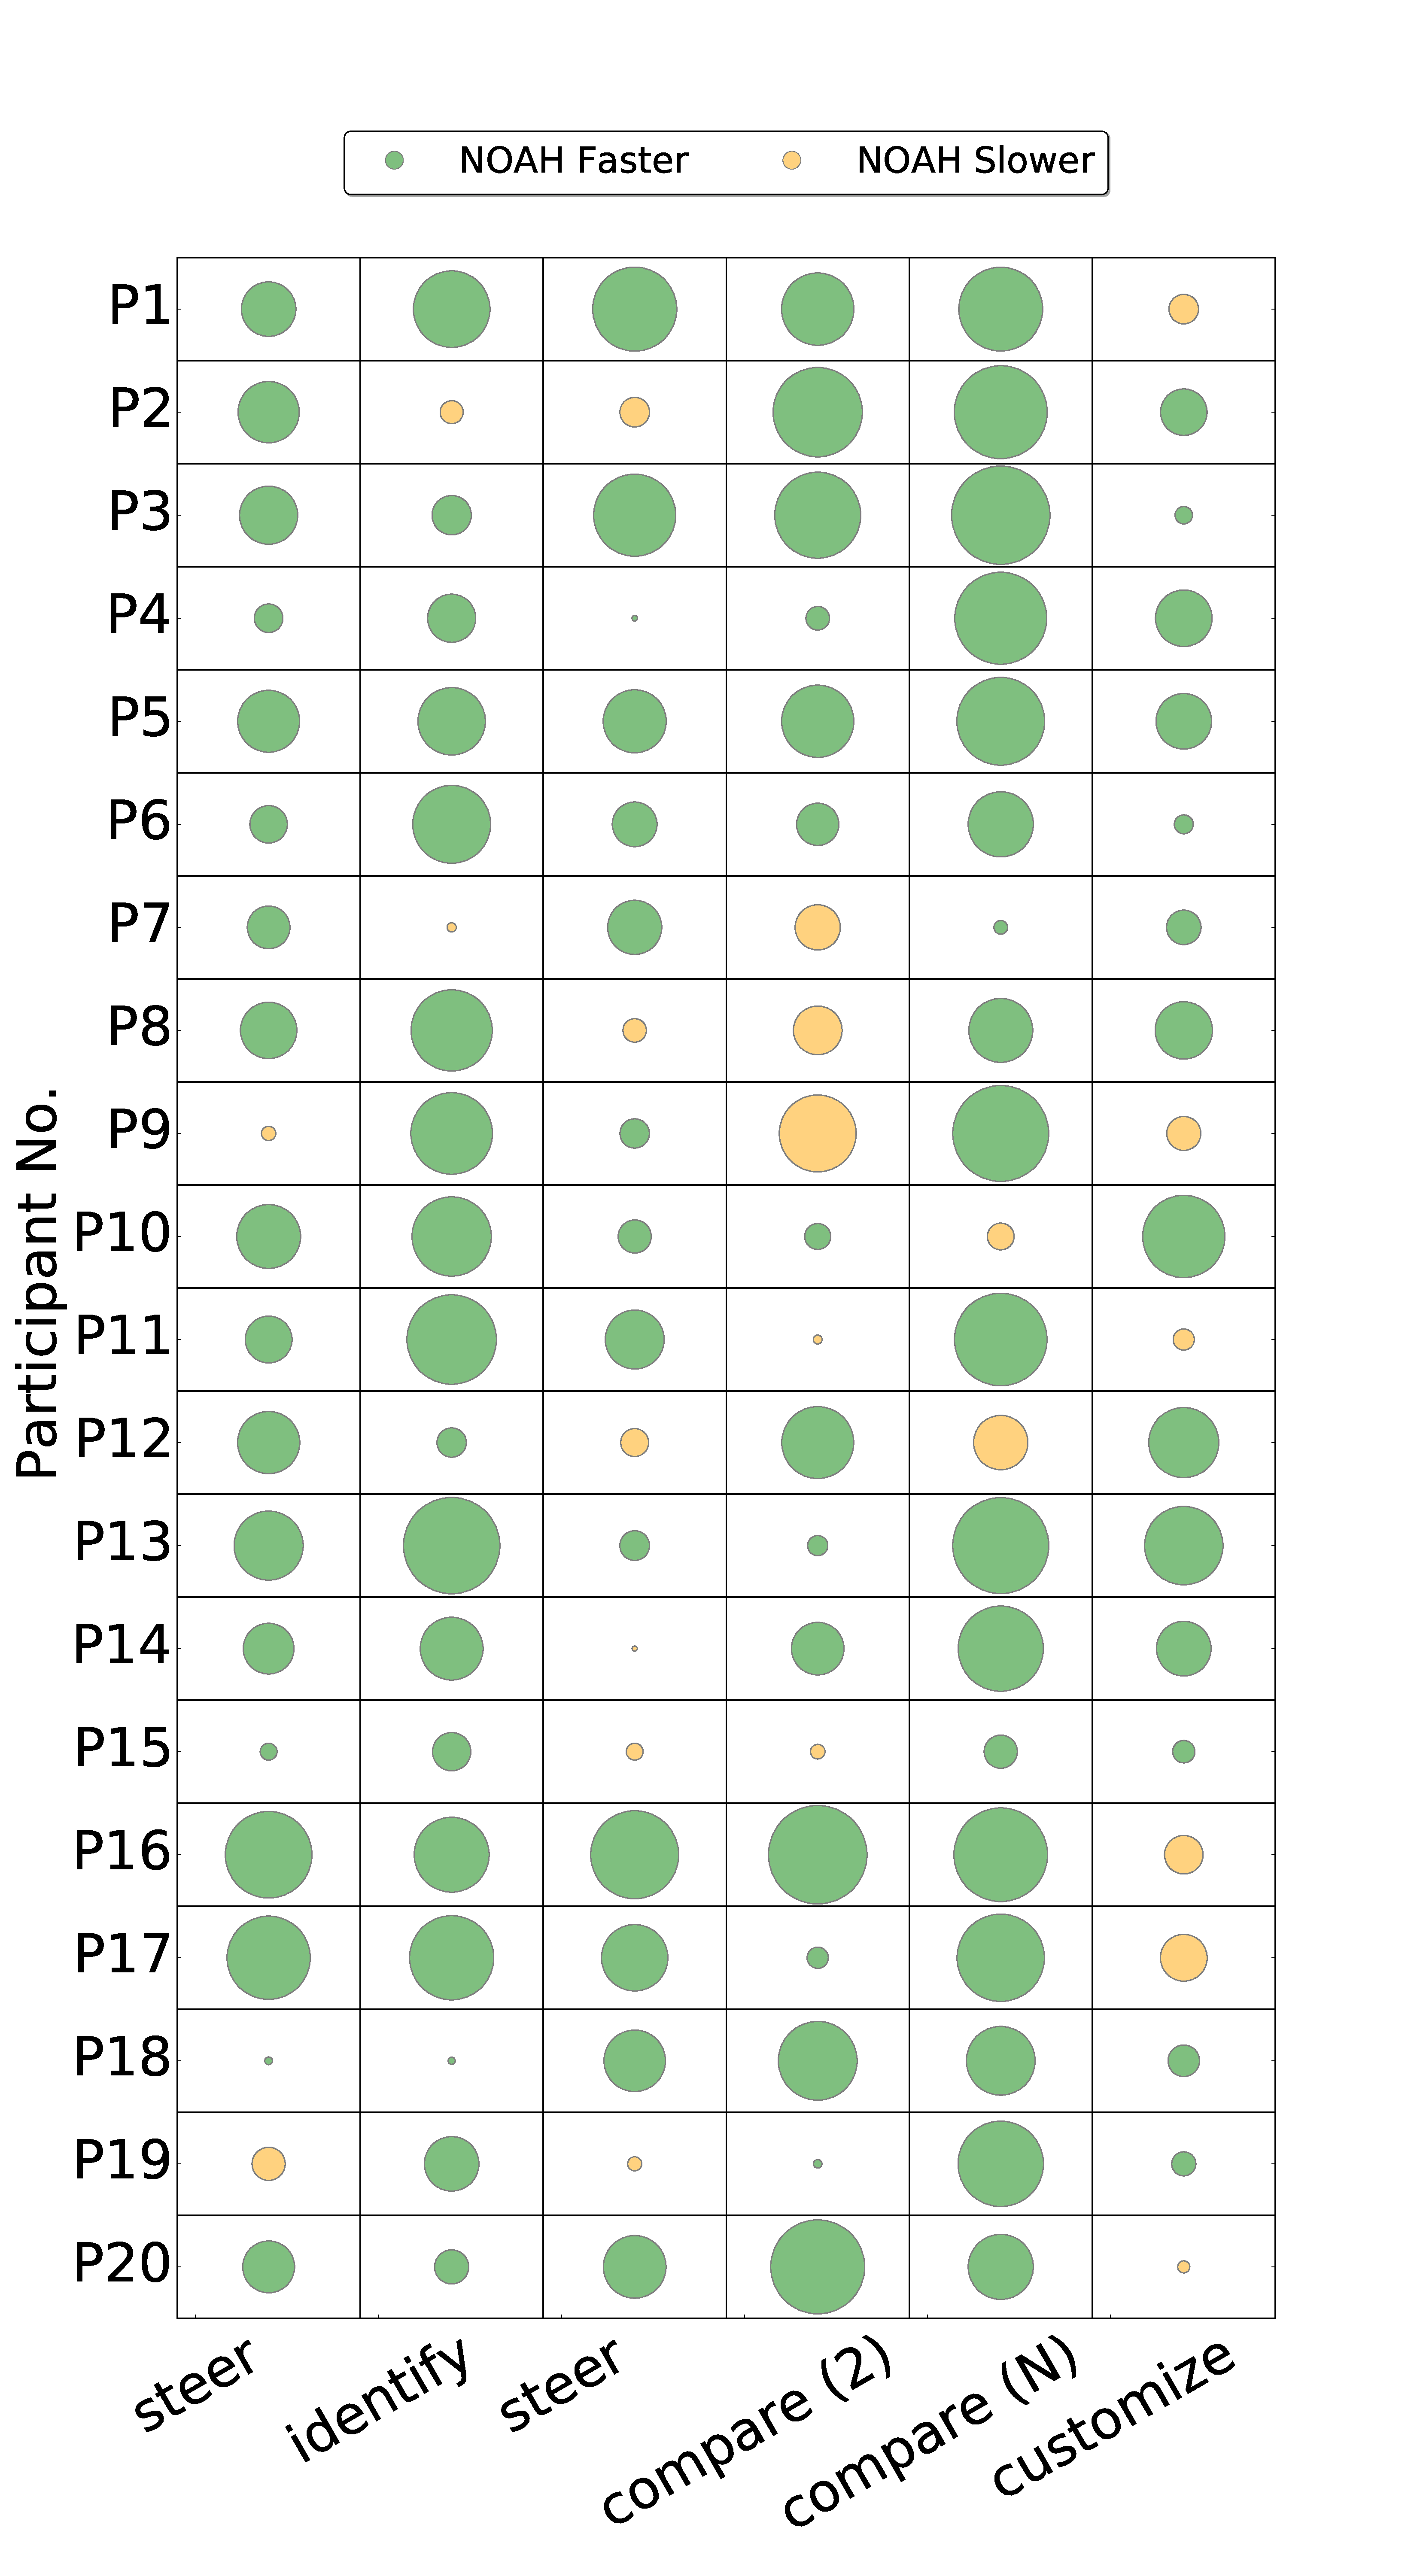
\includegraphics[trim=0 57 0 145,clip,width=\linewidth]{images/userinfo-ip-1.pdf}
   \caption{Intra-participant submission time differences between \noah and Excel across the quiz tasks.}
   \label{fig:ipdiff}
 \end{figure}

\subsection{Intra-participant differences.}
Figure~\ref{fig:ipdiff} depicts the intra-participant submission time differences between \noah and Excel, across all the quiz tasks.
For a given task and a participant, the corresponding circle denotes by what percentage (between $0.30\%$ to $94.33\%$) a system is faster than the competing system. The color of the circle denotes which system was faster (green: \noah faster, yellow: Excel faster). The larger the circle the faster the corresponding system is. For example, participant $P9$'s submission time was $91.78\%$ faster with \noah for the \cmpB task and $72.62\%$ faster with Excel for the \cmpA task. Figure~\ref{fig:ipdiff} confirms that majority of the submission times using \noah were faster compared to Excel---nineteen out of the twenty participants completed at least four tasks in less time using \noah compared to Excel. The submission time difference is even more apparent for the steer, identify, and \cmpB tasks.

For \cmpA, customize, and the second steer task, less than a third of the participants' submission times were faster using Excel. 
For the second steer tasks, four out of the six participants that submitted answers quickly using Excel compared to \noah, utilized the \emph{autosum} shortcut for the birdstrikes dataset. For the \cmpA tasks, a number of participants ($N=3$) that required more time to submit answer using \noah, first used the bin customization feature to view all the unique bins which contributed to the higher submission time compared to Excel. On the other hand, as explained earlier, the unfamiliarity with the bin customization feature contributed to higher submission time using \noah for six participants (yellow circles).

\subsection{Statistical Significance: Task Performance}
Since we conducted our user study on a small population (20 participants), we further evaluated the statistical significance of the task performance results, \ie accuracy and completion time. 
To measure the significance of the task completion times, we ran \emph{Mann-Whitney's U test} (as completion times did not follow a normal distribution). \emph{For all of the tasks except the customize task, we found a significant effect of the tools, \ie the response times for the tasks significantly differed by the choice of the tool} (see Table~\ref{tab:statTest}). 
On the other hand, we ran the \emph{Fisher's exact test} that measures the statistical significance of categorical data (0/1 accuracy): \emph{only for steer tasks, the percentage of the accuracy of submissions significantly differed by the choice of the tool}. 

\begin{table}[!htb]{}
\vspace{-10pt}
\scriptsize
\caption{Statistical significance of submission time and accuracy comparisons between \noah and Excel. (*) indicates statistically significant.}
\label{tab:statTest}
\centering
\begin{tabular}{cccc}
\hline
Question & Category &  Time   &    Accuracy \\
& & ($p$ value) & ($p$ value) \\ \hline
$Q1$ & Steer & $\mathbf{0.0007}$ (*) &  $\mathbf{0.0033}$ (*)  \\
$Q2$ & Identify &   $\mathbf{2.49 \times 10^{-5}}$ (*) & $0.7475$ \\  
$Q3$ & Steer & $\mathbf{0.0043}$ (*) & $\mathbf{0.0202}$ (*) \\
$Q4$  & \cmpA & $\mathbf{0.0154}$ (*) & $1$ \\  
$Q5$ & \cmpB & $\mathbf{5.83 \times 10^{-6}}$ (*) & $0.48$\\
$Q6$ & Customize & $0.1207$ &    $0.0959$ \\\hline
\end{tabular}
\vspace{-10pt}
\end{table}

\subsection{Statistical Significance: Subjective Ratings}
We further conducted a statistical significance test---the \emph{Wilcoxon Signed-rank} test---on the survey responses which showed that for all the metrics, the ratings significantly differed by the choice of the tool, \ie \noah or Excel. The distribution of the ratings for none of the criteria followed a normal distribution.

\begin{table}[!htb]{\scriptsize}
\caption{Survey results. (*) indicates statistical significance. }
\label{tab:survey}
\centering
\begin{tabular}{|l|l|l|l|}
\hline
Metric &    \noah   &    Excel   & $p$ value \\ \hline
Ease of Learning &  $\mu = 5.75$, &    $\mu = 4.22$, & $\mathbf{1.49 \times 10^{-7}}$ (*) \\
& $\sigma = 1.02$ & $\sigma = 1.41$ & \\\hline
Speed of Use &    $\mu = 6.03$, & $\mu = 4.22$, & $\mathbf{1.68 \times 10^{-7}}$ (*)\\
& $\sigma = 0.99$ & $\sigma = 1.65$ & \\\hline  
Ease of Use    & $\mu = 5.88$, & $\mu = 4.33$, & $\mathbf{7.85 \times 10^{-6}}$ (*) \\
& $\sigma = 0.90$ & $\sigma = 1.71$ & \\\hline
Confidence    & $\mu = 5.50$, & $\mu = 4.60$, & $\mathbf{0.0096}$ (*)\\
& $\sigma = 1.79$ & $\sigma = 1.50$ & \\\hline  
Comprehensibility & $\mu = 5.60$, & $\mu = 4.48$, & $\mathbf{0.0006}$ (*)\\
& $\sigma = 1.27$ & $\sigma = 1.65$ & \\\hline
Satisfaction & $\mu = 5.48$, &    $\mu = 4.52$, & $\mathbf{0.0018}$ (*)\\
& $\sigma = 1.16$ & $\sigma = 1.49$ & \\\hline
\end{tabular}
\end{table}


% that's all folks
\end{document}


